% Precompiled KV Memory Modules — arXiv preprint
% Build: tectonic main.tex   (XeTeX engine; UTF-8 native)
\documentclass[11pt]{article}

\usepackage[margin=1in]{geometry}
\usepackage{amsmath,amssymb}
\usepackage{booktabs}
\usepackage{array}
\usepackage{graphicx}
\usepackage{caption}
\usepackage{pdflscape}
\usepackage{microtype}
\usepackage{natbib}
\PassOptionsToPackage{hyphens}{url}
\usepackage[hidelinks]{hyperref}
\usepackage{url}

\captionsetup{font=small,labelfont=bf}
\setlength{\tabcolsep}{5pt}

\newcommand{\kmd}{\texttt{.kmd}}
\newcommand{\mdc}{\texttt{mdc}}
\newcommand{\code}[1]{\texttt{#1}}

\title{\textbf{Precompiled KV Memory Modules: Relocatable, Composable Agent Memory for LLM Inference Runtimes}\thanks{Code, data, and raw experimental outputs: \url{https://github.com/k0n1m4k1/kv-memory-modules}. Archived on Zenodo: \href{https://doi.org/10.5281/zenodo.21499493}{DOI:10.5281/zenodo.21499493} (all versions).}}
\author{Luis Andrés González Picazo}
\date{v1.0 --- July 21, 2026}

\begin{document}

\maketitle

\begin{abstract}
\noindent
Persistent memories for LLM agents are stored today as text files (Markdown) that are re-prefilled every session, or indexed in RAG systems that re-inject text fragments. The same holds for the skill, plan, and agent-definition files (\code{SKILLS.md}, \code{PLANS.md}, \code{AGENTS.md}) and the JSON tool schemas an agent loads, whether directly or over MCP: all of it is re-evaluated by the LLM on every new session and access --- compute time that consumes resources on every cold start. We propose treating each memory as a \textbf{precompiled KV module}: the attention state (per-layer K/V tensors) produced by evaluating the text once, serialized to disk with content-addressed identity, and \textbf{re-insertable at any position} of a live context via RoPE position re-rotation and sequence fusion --- without re-evaluating the text. Using stock llama.cpp release binaries, across nine instruction-tuned models (2B--14B; four full-attention, four linear-attention hybrids --- one carrying an MTP draft head --- and one interleaved sliding-window model) and memories up to 51.8k tokens, we demonstrate: (1) \textbf{non-prefix insertion with no statistically detectable recall difference} versus joint prefill (paired McNemar exact $p=0.69$; 95\,\% CI on the deficit $[-1.7, +3.1]$\,pp over 420 core paired questions, \S\ref{sec:single}), under adversarial prefixes, replicated bit-for-bit in recall across OS, GPU vendor, and backend (Windows/Vulkan/Arc vs.\ Linux/CUDA/RTX); (2) a setup-cost advantage that is a function of available compute --- restoring a 15.2k-token module from disk takes a flat ${\sim}0.7$\,s while prefilling it takes 5.5\,s on a discrete GPU, 13.7\,s under partial layer offload, and 18.9\,s on CPU (\textbf{7.0--27.6$\times$}, median of five runs) --- a ratio that also grows with model size (3.5$\times$ at 14B) and memory length (6.1$\times$ at 51.8k tokens) on the same GPU, and barely moves when the module is read cold from NVMe rather than the OS page cache (0.78\,s vs 0.65\,s at full GPU: state relocation dominates, not the disk) --- which makes precompilation most valuable precisely on consumer and edge hardware; (3) two-module composition with a characterized, statistically confirmed 10--20\,\% attribution deficit (pooled McNemar $p<0.001$), \textbf{reduced by recomputing ${\sim}\tfrac{1}{3}$ of the inserted module} (splice-$k$) and closing to parity at scale --- a 33.4k-token three-module workspace matches joint prefill (106 vs.\ 105 of 120; McNemar $p=1.0$); (4) lazy loading of \code{[[linked]]} modules mid-conversation ($0/6 \to 6/6$ after a 1.1\,s link of a 10.2k-token module); (5) \textbf{extension of the linker to linear-attention hybrids} (Qwen3.5 / Gated DeltaNet): recurrent state links as a constant-size affine pair $(T_M, S_M)$ extracted via per-layer probes with no runtime modification, reaching full recall parity with joint prefill at 2B, 4B and 9B; (6) a module ABI: KV-cache dtype is model- and length-dependent (q8\_0 matches f16; q4/q5 collapse silently on some models past ${\sim}9$k tokens), backend is \emph{not} a compatibility axis, modules are machine-portable artifacts, and interleaved sliding-window attention links unmodified --- the module inherits the window's own visibility semantics (\S\ref{sec:swa}); and (7) \textbf{compatibility with speculative decoding via multi-token-prediction (MTP) draft heads}: we identify the serialization gap that silently drops draft-head KV in llama.cpp, close it with a ${\sim}120$-line library patch, and show that restored state preserves draft acceptance (0.72 vs.\ 0.69 full-prefill baseline; removing only the draft blob degrades it to 0.59 with a 9\,\% throughput loss while answers stay correct). These results identify the ``memory linker'' --- absent today from both llama.cpp and vLLM --- as the missing piece for agent memory managers with near-zero warm-up cost. The linker is implemented and evaluated on llama.cpp; the vLLM result (E9) is a prefix-restore feasibility check and the cross-runtime \code{.kmd} format a proposal (\S\ref{sec:interchange}), not yet a demonstrated vLLM linker. To our knowledge, this is the first system to give KV state an \emph{artifact} lifecycle --- persistent, portable, content-addressed, staleness-checked --- rather than a cache-entry lifetime, the first KV linker of any kind for hybrid linear-attention models, and the first serialization of MTP draft-head KV state in a consumer runtime; everything runs on unmodified release binaries, with no engine fork, custom kernels, or fine-tuning (the sole exception is the \S\ref{sec:mtp} MTP result, which requires our upstream-candidate serialization fix --- vLLM needs none, \S\ref{sec:interchange}).
\end{abstract}

\subsection*{Resumen (Español)}
\noindent
Las memorias persistentes de los agentes LLM se almacenan hoy como archivos de texto (Markdown) que se reprocesan (\emph{prefill}) en cada sesión, o se indexan en sistemas RAG que reinyectan fragmentos de texto. Lo mismo ocurre con \code{SKILLS.md}, \code{PLANS.md}, \code{AGENTS.md} y la definición en JSON de las herramientas, sea de forma directa o por MCP: todo ello es reevaluado por el LLM en cada nueva sesión y acceso --- tiempo de cómputo que consume recursos en cada arranque en frío. Proponemos tratar cada memoria como un \textbf{módulo KV precompilado}: el estado de atención (tensores K/V por capa) resultante de evaluar el texto una sola vez, serializado a disco con identidad direccionada por contenido, y \textbf{re-insertable en cualquier posición} de un contexto vivo mediante re-rotación RoPE de posiciones y fusión de secuencias --- sin re-evaluar el texto. Sobre binarios oficiales de llama.cpp, con nueve modelos (2B--14B; cuatro de atención completa, cuatro híbridos de atención lineal ---uno de ellos con cabezal draft MTP--- y uno de ventana deslizante intercalada) y memorias de hasta 51,8k tokens, demostramos: (1) \textbf{inserción no-prefijo sin diferencia de recall estadísticamente detectable} frente al prefill conjunto (McNemar pareado exacto $p=0{,}69$; IC 95\,\% del déficit $[-1{,}7, +3{,}1]$\,pp sobre 420 preguntas pareadas, \S\ref{sec:single}), con prefijos adversarios, replicada con puntuaciones idénticas entre SO, fabricante de GPU y backend (Windows/Vulkan/Arc vs.\ Linux/CUDA/RTX); (2) una ventaja de coste de arranque que es función del cómputo disponible --- restaurar un módulo de 15,2k tokens desde disco cuesta ${\sim}0{,}7$\,s planos mientras su prefill cuesta 5,5\,s en GPU dedicada, 13,7\,s con offload parcial de capas y 18,9\,s en CPU (\textbf{7,0--27,6$\times$}, mediana de cinco ejecuciones) --- una razón que además crece con el tamaño del modelo ($\times$3,5 a 14B) y con la longitud de la memoria ($\times$6,1 a 51,8k tokens) en la misma GPU, y apenas se mueve aunque el módulo se lea en frío desde el NVMe en lugar de la page cache del SO (0,78\,s vs 0,65\,s a plena GPU: domina la relocación del estado, no el disco) --- lo que hace la precompilación más valiosa justo en hardware doméstico y de borde; (3) composición de módulos con un déficit de atribución del 10--20\,\% confirmado estadísticamente (McNemar $p<0{,}001$), \textbf{reducido recomputando ${\sim}\tfrac{1}{3}$ del módulo insertado} (splice-$k$) y con paridad recuperada a escala --- un workspace de 33,4k tokens y tres módulos iguala al prefill conjunto (106 vs.\ 105 de 120; McNemar $p=1{,}0$); (4) carga perezosa de módulos \code{[[enlazados]]} en mitad de la conversación ($0/6 \to 6/6$ tras un enlace de 1,1\,s de un módulo de 10,2k tokens); (5) \textbf{extensión del linker a híbridos de atención lineal} (Qwen3.5 / Gated DeltaNet): el estado recurrente se enlaza como par afín $(T_M, S_M)$ de tamaño constante extraído con sondas por capa sin modificar el runtime, con paridad total de recall en 2B, 4B y 9B; (6) un ABI de módulos: el dtype de la cache KV depende del modelo y la longitud (q8\_0 iguala a f16; q4/q5 colapsan silenciosamente en algunos modelos a partir de ${\sim}9$k tokens), el backend \emph{no} es eje de compatibilidad, los módulos son artefactos portables entre máquinas, y la atención de ventana deslizante intercalada enlaza sin modificación alguna --- el módulo hereda la semántica de visibilidad de la propia ventana (\S\ref{sec:swa}); y (7) \textbf{compatibilidad con la decodificación especulativa vía cabezales de predicción multi-token (MTP)}: identificamos el hueco de serialización que descarta silenciosamente el KV del cabezal draft en llama.cpp, lo cerramos con un parche de ${\sim}120$ líneas en la librería, y mostramos que el estado restaurado preserva la aceptación especulativa (0,72 vs.\ 0,69 de baseline con prefill completo; retirar solo el blob draft la degrada a 0,59 con $-9\,\%$ de throughput, con respuestas correctas). Los resultados sitúan el ``linker de memorias'' ---inexistente hoy en llama.cpp y vLLM--- como la pieza que falta para un gestor de memorias de agente con coste de arranque casi nulo. El linker está implementado y evaluado sobre llama.cpp; el resultado en vLLM (E9) es una comprobación de viabilidad de restauración prefijo y el formato \code{.kmd} entre runtimes una propuesta (\S\ref{sec:interchange}), no todavía un linker demostrado en vLLM. Hasta donde sabemos, este es el primer sistema que da al estado KV un ciclo de vida de \emph{artefacto} ---persistente, portable, direccionado por contenido, con verificación de obsolescencia--- en lugar de una vida de entrada de caché, el primer linker KV de cualquier tipo para modelos híbridos de atención lineal, y la primera serialización del estado KV de cabezales MTP en un runtime de consumo; todo sobre binarios oficiales sin modificar, sin forks del motor, kernels a medida ni fine-tuning (la única excepción es el resultado MTP de \S\ref{sec:mtp}, que requiere nuestra corrección de serialización candidata a upstream --- vLLM no necesita ninguna, \S\ref{sec:interchange}).

\section{Introduction}

Agent frameworks persist long-lived knowledge --- user preferences, project state, conventions --- as natural-language files (typically Markdown) injected into the context at session start; the same is true of the skill, plan, and agent-definition files (\code{SKILLS.md}, \code{PLANS.md}, \code{AGENTS.md}) and the JSON tool schemas an agent loads, directly or over MCP. This design pays the \emph{prefill tax} on every session: the same tokens are re-evaluated through the full transformer stack, at a cost that grows with memory size and model depth, on every cold start. Retrieval-augmented approaches reduce \emph{what} is injected but still re-evaluate whatever is retrieved.

The key observation is an analogy with managed runtimes: a Markdown memory is \emph{source code}; the KV-cache entries produced by prefilling it are its \emph{compiled form}; and the inference runtime is a \emph{virtual machine} that can, in principle, load compiled artifacts directly. Java does not re-run \code{javac} on every JVM start. This work asks: \textbf{can agent memories be compiled once into KV artifacts and linked into live contexts at arbitrary positions, across sessions, processes, and backends?}

Prefix caching (in llama.cpp, vLLM, and commercial APIs) already answers a restricted form of this question: compiled prefixes can be reused \emph{if and only if the new context starts with the exact same tokens}. This restriction is fatal for agent memory: any variable content before the memory --- a date, a greeting, a conversation turn --- invalidates the entire cached artifact (we quantify this in \S\ref{sec:phasea}). What is missing is the \textbf{linker}: relocation of a compiled module to a new position, and composition of independently compiled modules. Concurrent serving-side work addresses relocation for datacenter engines (position-independent caching, \S\ref{sec:related}); no linker ships in the runtimes themselves, and none covers persistent memory artifacts, consumer hardware, or hybrid architectures.

Contributions:

\begin{enumerate}
  \item A code-level analysis of KV persistence in llama.cpp and vLLM, identifying the existing primitives (serialization, RoPE K-shift relocation, sequence fusion) and the structural prefix-only constraint in both (\S\ref{sec:background}).
  \item A working memory linker for llama.cpp built entirely on public APIs of unmodified release binaries (\S\ref{sec:linker}).
  \item An experimental evaluation on four full-attention models (Qwen3-4B, Llama-3.2-3B, Qwen2.5-Coder-7B, Qwen3-14B) and memories from 1.4k to 51.8k tokens showing single-module insertion with no statistically detectable recall difference from joint prefill (\S\ref{sec:single}), a characterized multi-module attribution deficit that shrinks with model capability and is reduced by splice-$k$ recomputation (fully closed to parity at workspace scale, not at the two-module micro-scale), a 33.4k-token three-module workspace at parity with joint prefill, and a viable lazy-loading protocol for linked modules (\S\ref{sec:single}--\S\ref{sec:lazy}, \S\ref{sec:workspace}).
  \item An extension of the linker to linear-attention hybrids (Qwen3.5 at 2B/4B/9B, Gated DeltaNet): recurrent state linked as a constant-size affine pair extracted via per-layer probes, plus a host-side software RoPE rebase that removes the runtime's M-RoPE relocation restriction (\S\ref{sec:hybrid}).
  \item A cross-hardware, cross-runtime replication (Windows/Vulkan/Arc $\leftrightarrow$ Linux/CUDA/RTX; llama.cpp $\leftrightarrow$ vLLM) and a compute-regime cost model showing that the linker's $O(\text{bytes})$ advantage over prefill's $O(\text{compute})$ grows exactly where compute is scarce --- consumer CPUs and partial layer offload --- and additionally with model size and memory length, and does not depend on the module being cached in RAM: a cold NVMe read costs essentially the same as a warm one (${\sim}0.1$\,s more, \S\ref{sec:regimes}).
  \item A module ABI analysis (what breaks compatibility, including a model- and length-dependent KV-quantization cliff) and a runtime-agnostic interchange format proposal with content-addressed identity, implemented as the \kmd{} container and \mdc{} CLI (\S\ref{sec:abi}).
  \item Compatibility with MTP speculative decoding: a code-level identification of the draft-head serialization gap in llama.cpp (shared-cell KV state is silently dropped), a ${\sim}120$-line upstream-candidate fix, and a causal validation on a hybrid+MTP model --- restored state preserves draft acceptance, and ablating only the draft blob degrades it (\S\ref{sec:mtp}).
  \item A measured \textbf{context-virtual-memory layer} built from the same primitives: in-conversation eviction with compaction (0.5--1\,ms full-attention; ${\sim}5$\,ms checkpoint-and-replay for hybrids), sealing live conversation segments as relocatable modules (a 5.5k-token conversation lives in a 4k window with 142\,ms page-ins), and paged reading of a 51.8k-token document under a 4k budget that \emph{outscores} full-context prefill by 15 points (\S\ref{sec:byref}--\S\ref{sec:cvm}).
\end{enumerate}

Relative to the concurrent position-independent-caching line (\S\ref{sec:related}), four properties of this work are, to our knowledge, unique. First, \textbf{modules are artifacts, not cache entries}: compiled once, stored on disk with content-addressed identity, checked for staleness, and reused across sessions, processes, machines, and backends --- all measured, not assumed (\S\ref{sec:regimes}). Second, \textbf{the mechanism requires nothing from anyone}: unmodified release binaries of a consumer runtime, no engine fork, no custom kernels, no fine-tuning --- every ingredient already ships. Third, \textbf{architecture coverage}: this is the first KV linker for linear-attention hybrids, where a module becomes a constant-size affine operator on recurrent state (\S\ref{sec:hybrid}) --- arguably a more natural compiled memory than per-token KV. Fourth, \textbf{the economics are characterized, not just the mechanism}: the advantage is a function of compute scarcity (7.0--27.6$\times$ for the same module, \S\ref{sec:regimes}), peaking exactly on the consumer and edge hardware that serving-side systems do not target. Beyond mechanism, the evaluation contributes an empirical \emph{bound} on the phenomenon that approximation-based systems model: prefix-induced KV deviation is behaviorally negligible for single modules up to 15k tokens (no statistically detectable difference over 420 paired questions, \S\ref{sec:single}), and where it does matter --- multi-module attribution --- a small exact recomputation reduces it, closing to parity at workspace scale (\S\ref{sec:compose}, \S\ref{sec:workspace}).

\section{Related Work}
\label{sec:related}

\paragraph{KV state serialization and prefix reuse.}
llama.cpp exposes per-sequence state save/restore (\code{llama\_state\_seq\_*}) and server-level slot persistence; its RAM prompt cache reuses states by longest common prefix. vLLM \citep{kwon2023} implements Automatic Prefix Caching by addressing KV blocks with chained content hashes; SGLang's RadixAttention \citep{zheng2024} organizes reusable prefixes in a radix tree. vLLM's \code{KVConnectorBase\_V1} interface supports external KV stores --- LMCache \citep{lmcache2024}, Mooncake \citep{qin2025}, NIXL --- with asynchronous, layer-wise injection into paged memory. All of these reuse state only at identical prefix positions.

\paragraph{Modular and non-prefix reuse.}
Prompt Cache \citep{gim2024} proposed modular attention-state reuse with a schema of interchangeable segments. CacheBlend \citep{yao2025} fuses independently compiled KV chunks at non-prefix positions by selectively recomputing a small fraction of tokens, recovering most of the quality gap. CacheGen \citep{liu2024} compresses KV states for storage and transmission.

\paragraph{Position-independent caching (PIC).}
Non-prefix KV reuse has since crystallized into a named research area on the serving side: EPIC \citep{hu2025} formalizes PIC and mitigates the per-chunk attention-sink effect with static sparse recomputation; KVLink \citep{yangj2025} adjusts positional embeddings at concatenation time and fine-tunes the model with trainable link tokens; KVCOMM \citep{ye2025} \emph{estimates} prefix-induced cache deviation from an online pool of anchor examples; MiniPIC \citep{ordonez2026} hosts PIC primitives in a vLLM fork with under 100 lines of engine changes; and KEEP \citep{yangz2026}, closest in motivation, manages embodied-agent memory as KV cache groups inside one vLLM instance (${\sim}2.8$k LOC extension) --- an online cache manager whose entries are neither persisted, relocated, versioned, nor portable, for full-attention models only. All of this line lives inside modified serving engines and targets datacenter deployment; the four properties unique to this work are listed at the end of \S1, and the capability-by-capability gap is mapped in Table~\ref{tab:gap}.

\paragraph{Virtual context management.}
MemGPT \citep{packer2023} introduced the operating-system metaphor for agent memory: a bounded main context backed by external storage, with the model paging information in and out via function calls. That metaphor operates at the \emph{text} level --- paged-out content is summarized (lossily) or stored as text, and page-in re-prefills it, paying exactly the tax this work eliminates. vLLM's PagedAttention \citep{kwon2023} applies the same metaphor one level down, to the \emph{physical} layout of KV blocks in GPU memory, without extending what a sequence can address; engine-internal KV tiering (InfLLM-style memory units, KEEP's GPU/CPU groups) pages attention state but inside one modified serving process, with no persistence, relocation, or portability. Our modules supply the missing middle layer: page-in/page-out of \emph{compiled state} on stock runtimes, at exact-state fidelity and $O(\text{bytes})$ cost, with measured in-conversation eviction (\S\ref{sec:byref}) --- which turns MemGPT-style virtual context from a summarize-and-reprefill protocol into an actual page file for attention state. What gets extended is the \emph{addressable} context (bounded by storage); the resident attention window remains bounded by the trained context length.

\paragraph{Attention sinks and hybrid architectures.}
StreamingLLM \citep{xiao2024} showed that initial-position tokens act as attention sinks; module insertion changes what occupies the early positions a module ``grew up with'', and our sink-dropping ablations (\S\ref{sec:compose}) probe this directly. Gated DeltaNet \citep{yangs2025} is the linear-attention recurrence used by the Qwen3.5 hybrids to which \S\ref{sec:hybrid} extends the linker.

\paragraph{What exists, and what was missing.}
We are explicit about what this work does not invent: state serialization, RoPE relocation, sequence fusion, non-prefix insertion, and the virtual-memory metaphor all pre-exist, and this section credits each. The claim is the vacant cell, per capability (Table~\ref{tab:gap}). Each mechanism row pre-exists in some form; no prior system fills any entry of the last column, and no combination of them yields the artifact lifecycle that persistent agent memory needs. That combination --- not any single trick --- is the contribution.

\begin{landscape}
\begin{table}[p]
  \centering\small
  \setlength{\tabcolsep}{6pt}
  \caption{Capability map: closest prior art per capability, and the cell that was vacant.}
  \label{tab:gap}
  \begin{tabular}{p{3.4cm}p{4.4cm}p{5.2cm}p{8.2cm}}
    \toprule
    Capability & Closest prior art & Its scope & Missing until this work \\
    \midrule
    Non-prefix KV insertion & CacheBlend, EPIC, KVLink & inside modified/fine-tuned serving engines & on unmodified consumer release binaries, from native primitives (\S\ref{sec:linker}) \\
    KV persistence across requests & LMCache, Mooncake; llama.cpp session files & prefix-keyed cache entries inside one serving stack & content-addressed, staleness-checked \emph{artifacts}, relocatable and portable across machines and backends (\S\ref{sec:regimes}, \S\ref{sec:axes}) \\
    Virtual context / paging & MemGPT (text), PagedAttention (physical blocks) & summarize-and-reprefill; GPU block layout & paging of \emph{compiled state} at exact-state fidelity, with ms-scale measured eviction (\S\ref{sec:byref}) \\
    Modular prompt reuse & Prompt Cache & schema-fixed positions, custom implementation & schema-free relocation to arbitrary positions, no custom kernels (\S\ref{sec:linker}) \\
    Hybrid (linear-attention) state reuse & vLLM Mamba/GDN prefix snapshots & prefix-shaped, engine-internal & non-prefix linking as a constant-size affine operator --- the first KV linker for hybrids (\S\ref{sec:hybrid}) \\
    MTP draft-head KV & LMCache DeepSeek-MTP layers & prefix-shaped, datacenter stack & first serialization in a consumer runtime, causally validated, with an upstream-candidate fix (\S\ref{sec:mtp}) \\
    In-conversation eviction & KEEP (engine-internal importance groups) & online cache manager, no persistence or relocation & measured evict+compact on live conversations, attention and recurrent paths alike (\S\ref{sec:byref}) \\
    \bottomrule
  \end{tabular}
\end{table}
\end{landscape}

\section{Background: what the runtimes already provide}
\label{sec:background}

\paragraph{llama.cpp.}
A sequence's state is serialized as: prompt tokens, then per KV cell its absolute position and sequence ids, then per layer the raw K rows and V rows (\code{llama-kv-cache.cpp:1957-2200}; file container at \code{llama-context.cpp:3105}; all code references at tag b10068). On restore, \emph{physical} cells are re-allocated freely, but \emph{logical} positions are restored verbatim --- no relocation is applied at load. Separately, \code{llama\_memory\_seq\_add} marks per-cell position deltas and the next decode executes a K-shift graph that re-rotates K in place via RoPE, including for quantized caches (\code{llama-kv-cache.cpp:566, 1909}). V carries no positional information under RoPE and is untouched. Sequence membership can be copied cheaply between sequences in a unified KV buffer (\code{seq\_cp}/\code{seq\_rm}). \textbf{All linker ingredients exist; they are simply not connected.}

\paragraph{vLLM.}
{\sloppy
Block identity is a chained hash of (parent hash, block tokens, extra keys) (\path{kv_cache_utils.py:596}), so a block's identity encodes its entire prefix: prefix-only reuse is enforced \emph{structurally by the addressing scheme}, not incidentally. The connector API's scheduler contract (\code{get\_num\_new\_matched\_tokens}) asks how many tokens \emph{beyond the computed prefix} the connector can supply --- the contract itself is prefix-shaped. Non-prefix insertion therefore requires scheduler cooperation, not merely a new connector.\par}

\paragraph{Model-family constraints.}
MTP contexts in llama.cpp share KV cells with the target context and all state operations silently no-op on them (\code{[TAG\_KV\_CACHE\_SHARE\_CELLS]}): MTP speculation is incompatible with state restore today. Classic two-model speculation is compatible (draft state is saved separately). M-RoPE (vision-language) models are excluded by \code{seq\_add}'s single-position assertion; sliding-window attention and recurrent hybrids have partial-state semantics.

\paragraph{Recurrent state is affine --- so hybrid modules are constant-size.}
The newest hybrid linear-attention generation (e.g., Qwen3.5, where 3 of every 4 layers use Gated DeltaNet recurrence, \code{src/models/qwen35.cpp}) is outside the \emph{implemented} linker's reach --- recurrent state has no per-token entries to relocate --- but not outside its mathematical reach. Because these recurrences are linear in the state ($S_t = A_t S_{t-1} + B_t$), an entire module's effect is an affine operator: $S(P;M) = T_M \cdot S(P) + S_M$, with $T_M = \prod A_t$ and $S_M$ the module's zero-state response. A recurrent module is therefore a \emph{constant-size} artifact (one $d \times d$ matrix plus one state per layer/head, regardless of module length), and linking is one matmul per layer --- the same associativity that chunked-scan training algorithms already exploit, never yet externalized as a persistable artifact. Recurrent state is position-invariant, so no rebasing is even needed; the hybrid's full-attention layers link exactly as in \S\ref{sec:linker}.

Note that \emph{prefix-shaped} persistence for these families is already production practice: vLLM snapshots Mamba/GDN states at block boundaries for prefix caching (\code{mamba\_cache\_mode: "all"}), and LMCache serializes MTP-layer KV for DeepSeek-MTP models --- confirming that MTP and hybrid support are engineering gaps in llama.cpp, not mathematical ones. Sections \ref{sec:single}--\ref{sec:lazy} use standard-RoPE, full-attention decoder models; \textbf{\S\ref{sec:hybrid} implements and validates the affine-composition linker on Qwen3.5 hybrids}, working around the M-RoPE \code{seq\_add} exclusion with a host-side software rebase.

\section{The memory linker}
\label{sec:linker}

We implement compile, load, relocate, and fuse operations against unmodified llama.cpp b10068 release binaries, via Python \code{ctypes} bindings (${\sim}200$ lines).

\begin{itemize}
  \item \textbf{Compile} (\mdc{} step): tokenize the memory text, prefill it alone as sequence 0 at positions $0..n{-}1$, and serialize with \code{llama\_state\_seq\_save\_file}. The artifact is the \emph{module}.
  \item \textbf{Link} at position $P$ of a live context: \code{llama\_state\_seq\_load\_file} into an auxiliary sequence; optionally drop leading cells; \code{llama\_memory\_seq\_add(aux, -1, -1, P)} to rebase positions (the RoPE K-shift executes lazily on the next decode); \code{seq\_cp}(aux $\to$ main) and \code{seq\_rm}(aux) to fuse. Requires \code{kv\_unified=true} and \code{n\_seq\_max} $\geq 2$.
  \item \textbf{ABI pinning}: flash attention is pinned off because \code{v\_trans = !flash\_attn} changes the serialized V layout; the KV dtype is pinned to f16 for the \S\ref{sec:single}--\S\ref{sec:lazy} experiments (both axes are explored systematically in \S\ref{sec:abi}, including all nine cache dtypes and an FA$\leftrightarrow$non-FA converter).
\end{itemize}

The linker adds ${\sim}0.4$--$0.6$\,s per link for 31--297\,MB modules on our hardware, dominated by disk I/O; the K-shift itself is a single fused graph pass.

\begin{figure}[t]
  \centering
  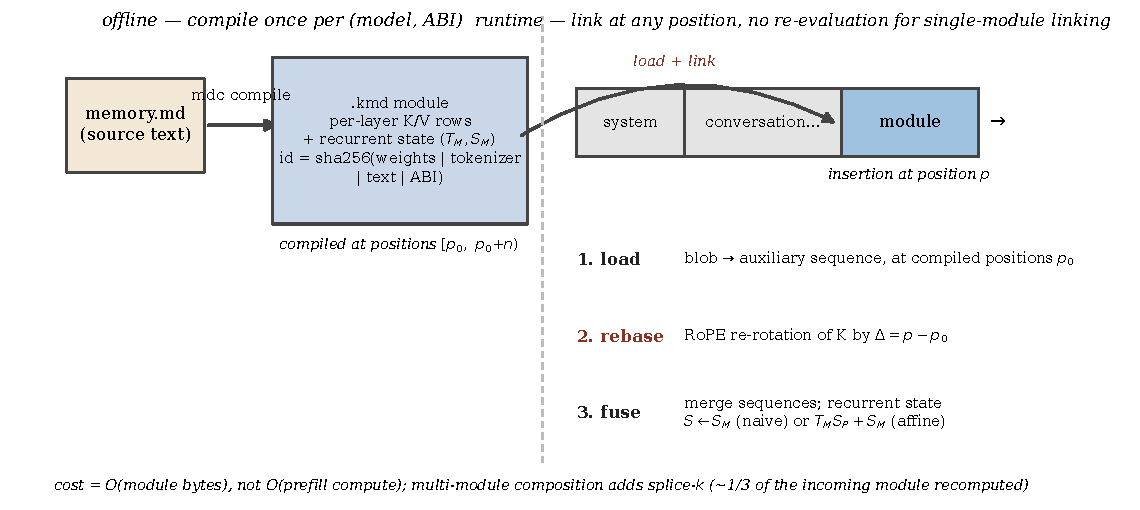
\includegraphics[width=\linewidth]{fig-linker.pdf}
  \caption{The memory linker. Left: a Markdown memory is compiled once per (model, ABI) into a content-addressed \kmd{} module holding per-layer K/V rows (plus, for hybrids, the recurrent-state pair). Right: at runtime the module is linked at an arbitrary position of a live context in three steps --- load, RoPE position rebase, sequence fusion --- with no re-evaluation of the text for single-module linking (multi-module composition additionally recomputes a splice-$k$ fraction of the incoming module, \S\ref{sec:compose}).}
  \label{fig:linker}
\end{figure}

\section{Experiments}
\label{sec:experiments}

\paragraph{Experiment map.}
Experiments are numbered in the order they were run; Table~\ref{tab:map} maps them to sections and scripts (all under \code{experiments/} in the repository).

\begin{table}[h]
  \centering\footnotesize
  \setlength{\tabcolsep}{4pt}
  \caption{Experiment map.}
  \label{tab:map}
  \begin{tabular}{llll}
    \toprule
    Exp & Section & What it measures & Script \\
    \midrule
    Phase A & \S\ref{sec:phasea} & Cold restore vs.\ prefill; prefix fragility & \code{scripts/run-poc*.ps1} \\
    E1, E2 & \S\ref{sec:single} & Single-module non-prefix insertion (short/adversarial prefix) & \code{bateria2.py} \\
    E8 & \S\ref{sec:single} & Scale check: 5.1k-token memory, $N{=}60$ (incl.\ the 14B point) & \code{bateria6.py} \\
    E3, E5 & \S\ref{sec:compose} & Two-module composition; splice-$k$ repair & \code{bateria2.py}, \code{bateria4.py} \\
    E4a, E4b & \S\ref{sec:lazy} & Lazy loading of linked modules & \code{bateria3.py}, \code{bateria3b.py} \\
    E7 & \S\ref{sec:hybrid} & Hybrid (GDN) linking, affine vs.\ naive & \code{hibrido2.py}--\code{hibrido4.py} \\
    E8-rep, E9 & \S\ref{sec:regimes} & Cross-machine replication; vLLM restore & \code{bateria6.py}, \code{fase3\_vllm.py} \\
    E10, E12 & \S\ref{sec:regimes} & 8--15k corpus from disk; regime sweep + cold-NVMe restore & \code{bateria7.py}, \code{e12.py} \\
    E14 & \S\ref{sec:regimes} & The 51.8k-token memory point, f16/q8\_0 dtype ablation & \code{e14.py} \\
    E11 & \S\ref{sec:workspace} & 33.4k-token multi-module workspace; lazy at scale & \code{bateria8.py} \\
    E13 & \S\ref{sec:mtp} & MTP speculative decoding over restored KV state & \code{e13v2.py} \\
    E6 & \S\ref{sec:dtype} & KV dtype ABI sweep & \code{bateria5.py} \\
    E15, E15b & \S\ref{sec:byref} & Live in-conversation eviction (full-attn.; hybrid ckpt+replay) & \code{e15.py}, \code{e15b.py} \\
    E16 & \S\ref{sec:cvm} & Conversational virtual memory: seal / archive / page-in & \code{e16.py} \\
    E17 & \S\ref{sec:limitations} & Two-hop recall over a linked module (three models) & \code{e17.py} \\
    E18 & \S\ref{sec:cvm} & Paged reading of the 51.8k-token document, 4k budget & \code{e18.py} \\
    E20 & \S\ref{sec:swa} & SWA (Gemma 3): link/rebase on the iSWA cache, window semantics & \code{bateria2.py}, \code{bateria6.py} \\
    \bottomrule
  \end{tabular}
\end{table}

\paragraph{Setup.}
\begin{itemize}
  \item \textbf{Machines.} A: Windows 11, Intel Arc 140V (16\,GB, Vulkan), llama.cpp b10068 official binaries. B (replication, \S\ref{sec:regimes}): Ubuntu 24.04, RTX 4070 Ti SUPER (16\,GB, CUDA), 20-core CPU, same tag built from source, plus vLLM 0.22.1 for E9.
  \item \textbf{Models.} Qwen3-4B-Instruct-2507 Q4\_K\_M (36 layers, GQA 8, f16 KV $\approx 147$\,KB/token), Llama-3.2-3B-Instruct Q4\_K\_M, Qwen2.5-Coder-7B-Instruct Q4\_K\_M (a scale and specialization point), and Qwen3-14B Q4\_K\_M (the largest full-attention point, \S\ref{sec:single}); \S\ref{sec:hybrid} adds the hybrids Qwen3.5-2B/4B Q4\_K\_M and Qwen3.5-9B Q8\_0 (ChatML harness with the thinking mode pinned off --- see the methodological note there); \S\ref{sec:mtp} adds Qwopus3.5-4B-Coder-MTP Q6\_K, a GDN hybrid with an embedded MTP draft head; \S\ref{sec:swa} adds Gemma-3-4B-it Q4\_K\_M (interleaved sliding-window attention). Full model properties and sources in Appendix~\ref{app:models}.
  \item \textbf{Decoding and scoring.} Greedy decoding throughout. Recall is scored by accent-insensitive substring match against facts that exist \emph{only} in the memory text, verified by no-memory controls.
  \item \textbf{Corpora.} \S\ref{sec:single}--\S\ref{sec:lazy} use a synthetic 1.4k-token project memory and a 0.3k-token secondary memory; E8 uses a deterministic 5.1k-token generated memory (seeded generator in the script); E10--E12 use three Wikipedia-bulk memories (8.0k/10.2k/15.2k tokens) whose questions target \emph{injected synthetic facts only} (fake expedient ids, assignees, budgets --- absent from any pretraining corpus by construction; seeded generator \code{gen\_corpus.py}), so parametric knowledge cannot inflate scores.
  \item \textbf{Isolation and hygiene.} Each question is asked from an identical base state, isolated by KV rollback (\code{seq\_rm}) --- we found and corrected a question-chaining confound that initially masqueraded as an insertion-quality deficit. Modules are recompiled per run and tagged per model; every link asserts the expected \code{seq\_pos\_max}.
\end{itemize}

\subsection{Cold restore vs.\ prefill, and prefix fragility (Phase A)}
\label{sec:phasea}

Single module restored as a prefix through the llama.cpp server's slot-persistence API --- the baseline the rest of the paper builds on.

\begin{table}[h]
  \centering\small
  \caption{Phase A: cold restore vs.\ full prefill (same module file on both backends).}
  \begin{tabular}{lcc}
    \toprule
    Metric & GPU (Vulkan) & CPU (same module file) \\
    \midrule
    Cold restore (1380 cells, 194\,MB) & 288\,ms & 358\,ms \\
    Query after restore & 46 tok / 218\,ms & 46 tok / 671\,ms \\
    Cold baseline (full prefill) & 1425 tok / 2196\,ms & 1425 tok / 8668\,ms \\
    TTFT speedup & \textbf{4.3$\times$} & \textbf{8.4$\times$} \\
    \bottomrule
  \end{tabular}
\end{table}

Outputs are token-identical to the baseline. The same binary artifact restores across backends: serialization copies raw host-side bytes (\code{ggml\_backend\_tensor\_get/set}), so the format is backend-agnostic (Vulkan/CUDA/SYCL/CPU); the empirical Vulkan$\to$CPU transfer confirms it.

\paragraph{Prefix fragility.}
With a 47-token variable prefix (system + timestamp) prepended, the restored module contributes nothing: 1464/1464 tokens are reprocessed. One edited line in the source MD likewise invalidates everything after the divergence point. This is the problem the linker solves.

\subsection{Single-module insertion (E1, E2, E8)}
\label{sec:single}

\emph{Joint} = full prefill reference; \emph{naive} = linker insertion after the prefix. E1 asks $N{=}20$ memory-recall questions over a 47-token prefix; E2 asks $N{=}25$ (20 memory + 5 prefix-recall) over an adversarial ${\sim}1$k-token prefix --- a realistic assistant conversation containing same-type distractors (other URLs, other schedules, other ticket ids) for the memory facts. Cells show joint / naive; the control column lists the no-memory score per model (Qwen $\cdot$ Llama $\cdot$ Coder).

\begin{table}[h]
  \centering\small
  \caption{E1/E2: single-module insertion, joint / naive.}
  \begin{tabular}{lcccc}
    \toprule
    Experiment & Qwen3-4B & Llama-3.2-3B & Coder-7B & no-memory control \\
    \midrule
    E1: short prefix ($N{=}20$) & 17 / \textbf{18} & 20 / \textbf{19} & 20 / \textbf{20} & 5 $\cdot$ 1 $\cdot$ 4 \\
    E2: adversarial 1k prefix ($N{=}25$) & 23 / \textbf{23} & 23 / \textbf{24} & 24 / \textbf{24} & 4 $\cdot$ 8 $\cdot$ 9 \\
    \bottomrule
  \end{tabular}
\end{table}

\textbf{Insertion is indistinguishable from joint prefill in all three models} ($\pm 1$ = noise: failure sets are identical across conditions and shared with the reference; the 7B achieves perfect parity at 20/20 and 24/24). The theoretically expected cross-attention deficit --- module K/V never attended the prefix --- does not manifest at this scale, even under adversarial interference. Sink-dropping and 64-token warm-splice ablations neither help nor hurt (18/20 each on Qwen E1), consistent with there being no deficit to repair. Setup latency usually favors the linker (e.g., E2 Qwen: 2.2\,s vs 3.4\,s; E1 Coder: 0.6\,s vs 1.9\,s), with one observed inversion (E2 Coder: 5.1\,s vs 3.9\,s): the advantage is I/O-bound versus compute-bound and thus hardware- and size-dependent, growing with module length.

\paragraph{Scale check (E8).}
A deterministic synthetic memory of 5{,}114 tokens (40 microservices $\times$ 10 unique attributes + 20 incidents; generator and seed in \code{bateria6.py}) with an adversarial 1k-token prefix and \textbf{$N{=}60$} questions, on Qwen3-4B: joint 51/60, \textbf{linked 50/60}, no-memory control 0/60. Eight of the ${\sim}10$ failures are shared between conditions and the rest are same-type noise (the most confusable attribute across 40 services). Two properties strengthen with scale: the task is no longer saturated (85\,\% joint), so a deficit had room to appear and did not; and the setup advantage widens exactly as the $O(\text{bytes})$-vs-$O(\text{compute})$ argument predicts --- \textbf{1.7\,s linked vs 12.1\,s prefill (7.1$\times$)}, up from 3.1$\times$ at 1.4k tokens. Module weight becomes operationally relevant at this size (754\,MB at f16; ${\sim}400/210$\,MB at q8\_0/q4\_0 per \S\ref{sec:abi}, quality-free on this workload).

\paragraph{The 14B point.}
The same battery on Qwen3-14B Q4\_K\_M (machine B, full GPU) reaches \textbf{exact parity at a higher absolute score: joint 57/60, linked 57/60}, no-memory 0/60 --- the insertion deficit still fails to appear as model capacity grows, consistent with \S\ref{sec:compose}'s observation that the composition deficit \emph{shrinks} with capability. The setup advantage also grows with model size on identical hardware: \textbf{0.82\,s linked vs 2.87\,s prefill (3.5$\times$)}, versus 1.7$\times$ for the 4B on the same GPU --- prefill cost scales with model depth and width while restore remains a byte copy (838\,MB module), adding a third axis (model size, alongside compute regime and memory length) to the \S\ref{sec:regimes} economics.

\paragraph{Pooled significance.}
Individual cells here are underpowered ($N=10$--60); no single cell reaches significance in either direction. The claim of no insertion penalty therefore rests on the \emph{pool}. Aggregating every single-module battery (E1, E2, E8/E8-rep across the applicable models) into one paired test --- \textbf{420 paired questions} --- linked insertion scores 78.6\,\% against joint prefill's 79.3\,\%: \textbf{no statistically detectable difference} (McNemar exact $p=0.69$), with a 95\,\% Newcombe confidence interval on the joint$-$linked deficit of $\mathbf{[-1.7, +3.1]}$\,\textbf{pp}, inside a 10\,pp non-inferiority margin (we fix that margin \emph{post hoc}, having not pre-registered it --- an honest caveat). Extending the pool to the harder long-context and two-hop batteries (E14, E17; 600 questions total) leaves the verdict unchanged ($\Delta$ $+0.2$\,pp, $p=1.0$). This replaces the earlier ``no measurable loss'' wording with a bounded, testable statement; the analysis recomputes from the versioned per-question outputs (\code{experiments/stats\_recall.py}).

\subsection{Two-module composition and the splice-$k$ repair (E3, E5)}
\label{sec:compose}

Modules A (1.4k tok) and B (0.3k tok) compiled independently and linked in sequence; $N{=}10$ questions per module.

\begin{table}[h]
  \centering\small
  \caption{E3: two-module composition.}
  \begin{tabular}{lccc}
    \toprule
    Condition & Qwen3-4B & Llama-3.2-3B & Coder-7B \\
    \midrule
    joint (all prefilled) & 18/20 & 20/20 & 20/20 \\
    composed (A then B linked) & 16/20 & 16/20 & 18/20 \\
    \bottomrule
  \end{tabular}
\end{table}

The deficit (${\sim}10$--20\,\%) replicates across all three models, shrinks with model capability ($-2$ at 7B vs $-4$ at 3B against a perfect 20/20 base), and --- pooled across models ($N=140$ paired questions) --- is statistically robust, unlike the single-module case: \textbf{McNemar exact $p<0.001$, 95\,\% CI on the deficit $[+7.4, +20.5]$\,pp}. It has a specific signature: \textbf{cross-module attribution confusion} --- e.g., asked for module B's database, the composed condition answers with module A's (PostgreSQL instead of SQLite). Modules never attended each other; under interference, fact-to-scope binding weakens. Per-module scoring shows the deficit lives entirely in the \emph{later-linked} module: module A recall never degrades.

\paragraph{Boundary recomputation repairs it (E5).}
We evaluated fresh-decoded scope separators, recomputing the first $k$ tokens of module B in context (splicing the precompiled remainder via \code{drop\_k} linking), and their combination. Scores are module-B recall ($N{=}10$):

\begin{table}[h]
  \centering\small
  \caption{E5: splice-$k$ repair, module-B recall.}
  \begin{tabular}{lccc}
    \toprule
    Condition & Qwen3-4B & Llama-3.2-3B & Coder-7B \\
    \midrule
    joint (reference) & 10 & 10 & 10 \\
    composed, naive & 8 & 6 & 8 \\
    scope separators & 7 & 7 & 8 \\
    splice $k{=}32$ (${\sim}11\,\%$) & 7 & 8 & 7 \\
    \textbf{splice $k{=}96$ (${\sim}33\,\%$)} & 7 & \textbf{9} & \textbf{9} \\
    separators + splice32 & 6 & 7 & 7 \\
    \bottomrule
  \end{tabular}
\end{table}

Recomputing ${\sim}\tfrac{1}{3}$ of the inserted module moves module-B recall back toward the reference on the two models with a clear deficit (Llama: monotonic in $k$, $6 \to 8 \to 9$; Coder: $8 \to 9$), at the cost of prefilling 96 tokens --- negligible. Separators alone contribute little. On Qwen3-4B the composed deficit was already within noise and no fixup moves it. \textbf{These per-condition cells are $N=10$ and individually non-significant; pooled across models at $N=20$/condition, splice-$k$ \emph{reduces but does not fully close} the two-module deficit (repaired 81.7\,\% vs joint 95.0\,\%, still McNemar $p=0.039$).} The clean, powered parity result for the composition recipe is at workspace scale (\S\ref{sec:workspace}: $N=120$, $p=1.0$), not at this micro-benchmark. This is an in-situ confirmation of CacheBlend's thesis, implemented with nothing but rollback and offset linking. \textbf{Production recipe}: naive linking for single modules; splice-$k$ with $k \approx 33\,\%$ of the inserted module for multi-module composition --- whose quality-preserving parity is established at scale in \S\ref{sec:workspace}.

\subsection{Lazy loading of linked modules (E4a, E4b)}
\label{sec:lazy}

Full ``classloader'' scenario: a ${\sim}1$k-token agent system prompt is prefilled; a 2.1k-token \emph{general} memory module (containing the reference \code{[[memoria-ancla]]}) is linked after it; questions about the secondary project trigger loading the 0.3k-token linked module mid-conversation. General-memory recall on this linked base is 8/10 (Qwen3-4B), 9/10 (Llama-3.2-3B), and 9/10 (Coder-7B). We test two protocols: \textbf{E4a} links the module \emph{after} the question has already been decoded; \textbf{E4b} (\emph{load-then-requestion}) rolls back the ${\sim}20$-token question, links the module, and re-decodes the question after it (${\sim}0.5$\,s total). $N{=}10$ per condition:

\begin{table}[h]
  \centering\small
  \caption{E4: lazy loading protocols.}
  \begin{tabular}{lccc}
    \toprule
    Condition & Qwen3-4B & Llama-3.2-3B & Coder-7B \\
    \midrule
    joint (reference) & 10/10 & 10/10 & 10/10 \\
    E4a: module inserted after the question & 3/10 & 7/10 & 5/10 \\
    E4b: \textbf{load-then-requestion} & \textbf{8/10} & 6/10 & \textbf{9/10} \\
    no-load control & 1/10 & 3/10 & 3/10 \\
    \bottomrule
  \end{tabular}
\end{table}

Question-before-evidence ordering degrades every model (worst on Qwen3-4B, which answers ``this is not in the memory'', anchored on the general module's delegation statement). Load-then-requestion restores natural reading order and recovers accuracy to near-reference (9/10 on the 7B). The residual gap to 10/10 matches the E3 attribution deficit. Note that in a production agentic loop the requestion step is unnecessary: a model that defers its answer until after a tool result --- the standard tool-use pattern --- generates \emph{after} the link, so causal attention already sees the module (\S\ref{sec:skills}).

\subsection{Hybrid-model linking: Qwen3.5 / Gated DeltaNet (E7)}
\label{sec:hybrid}

We validate the affine-composition linker of \S\ref{sec:background} on Qwen3.5-2B (Q4\_K\_M), a hybrid with 18 of 24 layers using Gated DeltaNet recurrence (per-layer state: 16 heads $\times$ $128 \times 128$ f32, a \emph{fixed} ${\sim}20$\,MB per sequence regardless of context length) and 6 full-attention M-RoPE layers --- entirely in Python over unmodified release binaries (\code{hibrido2.py}).

\paragraph{Mechanics.}
\begin{enumerate}
  \item Whole-state save/restore (\S\ref{sec:phasea}-style, attention + recurrent) already works for hybrids: restored continuations are token-identical, so \emph{prefix-shaped} modules for Qwen3.5 need nothing new.
  \item \code{llama\_memory\_seq\_add} asserts \code{n\_pos\_per\_embd()==1} and is therefore unavailable for M-RoPE models: we replace the on-device K-shift with a \textbf{software rebase} --- a NEOX delta-rotation of the serialized K rows applied host-side (for text, all four M-RoPE sections carry the same position, so M-RoPE $\equiv$ NEOX; the same equivalence llama.cpp's own shift graph relies on), plus patching cell positions in the blob metadata. Verified against direct compilation at the target position: max K error $7.7 \times 10^{-2}$ (f16 double-rounding, not an algebra error). The linker thus requires \emph{no} runtime position support at all.
  \item The \code{PARTIAL\_ONLY} state flag gives read/write access to just the recurrent section of the hybrid state.
\end{enumerate}

\paragraph{Affine extraction without a custom graph pass.}
$S_M$ is the module's zero-state response (one normal compile). $T_M$ is extracted with \textbf{one probe per recurrent layer}: initialize layer $\ell$'s state to the identity and all other layers to zero --- shallower layers then behave exactly as in the compile pass, so layer $\ell$ sees its exact compile-time inputs, and since the per-layer map is exactly affine given its inputs, $T_M[\ell] = \text{probe}[\ell] - S_M[\ell]$ with no $\varepsilon$-truncation error. Probing a random state against the affine prediction gives $4$--$7 \times 10^{-3}$ relative error (an orientation mistake would give $O(1)$). Compile cost is $\times(L_{\text{recr}}+1)$ --- 1282 tokens $\to$ 2\,s base + 21\,s probes, offline. The per-layer artifact is \emph{constant-size}: $T$ (1\,MB) + $S_M$ (1\,MB) per layer for the 2B.

\paragraph{Results}
(E1-style battery, ChatML harness; recurrent rollback is not supported so per-question isolation uses a \code{seq\_cp} checkpoint sequence). Cells show memory recall + prefix recall:

\begin{table}[h]
  \centering\footnotesize
  \setlength{\tabcolsep}{3.5pt}
  \caption{E7: hybrid linking on Qwen3.5-2B.}
  \begin{tabular}{lcccc}
    \toprule
    Scenario & joint & naive ($S{:=}S_M$) & affine ($T_M S_P + S_M$) & no-mem \\
    \midrule
    1: 45-tok prefix + 1282-tok module (20q + 2q) & 20/20 + 2/2 & \textbf{20/20 + 2/2} & \textbf{20/20 + 2/2} & 4/20 + 1/2 \\
    2: ${\sim}1.1$k-tok prefix + 294-tok module (10q + 6q) & 10/10 + 5/6 & \textbf{10/10 + 6/6} & \textbf{10/10 + 6/6} & 1/10 + 6/6 \\
    \bottomrule
  \end{tabular}
\end{table}

Non-prefix insertion into a hybrid reaches \textbf{full recall parity with joint prefill} in both scenarios, under both recurrent-state policies. The result replicates exactly on Qwen3.5-4B (32 layers, 24 recurrent): 20/20+2/2 and 10/10+6/6 across joint/naive/affine, and an ablation that compiles the module directly at the target position (no software rebase) also scores 20/20+2/2 under both policies --- attributing zero behavioral cost to the software rebase (max f16 K error $1.9 \times 10^{-1}$) and to the affine term alike. A second replication at 9B (Q8\_0 weights) appears in \S\ref{sec:regimes}.

State-space diagnostics separate the policies where the battery does not: relative $L_2$ distance from the joint state is 0.379--0.410 (naive) vs 0.266--0.289 (affine) with the short module, ${\sim}0.20$ vs ${\sim}0.19$ with the long one --- the affine term recovers real prefix-state information, and matters more the shorter the module (GDN's contractive gating decays $T_M \cdot S_P$ over long modules, making naive converge to affine). Link cost: 95--680\,ms naive, 0.65--2.0\,s affine.

We actively searched for a regime where the policies separate \emph{behaviorally} and did not find one: placing eight session facts immediately before the link point (maximal recency, hence maximal expected reliance on recurrent state) still yields 8/8 recall under naive on both module lengths --- the hybrid's full-attention layers (1 in 4) fully cover what naive discards from the prefix's recurrent state. The one recall failure observed is a prefix$\leftrightarrow$module \emph{attribution} confusion shared by both policies (the \S\ref{sec:compose} deficit class, a splice-$k$ candidate), not a state-policy effect. \textbf{Naive state replacement is therefore the production recommendation for GDN hybrids} (cheaper, no $T$ matrices in the module); the affine machinery is validated numerically and reserved for \emph{purely recurrent} models (Mamba/RWKV without full-attention layers), where it is the only mechanism that can preserve the prefix at all --- a natural next testbed. This closes the hybrid frontier of \S\ref{sec:background}: the compatible set now includes GDN hybrids.

\paragraph{A methodological trap worth reporting.}
Our first 4B run showed an apparent degradation (naive 16/20, affine 11/20 --- \emph{below} naive) that was entirely a harness artifact: every failed answer was \emph{empty}, because the thinking-mode model spent the whole generation budget inside an unclosed \code{<think>} block. Pre-filling the assistant turn with an empty think block (\code{<think>\textbackslash n\textbackslash n</think>}) restored full parity. Linked-state conditions can make a reasoning model \emph{think longer}, which under a token cap masquerades as a quality deficit --- batteries over thinking-capable models must pin the thinking mode or budget for it.

\subsection{Cross-hardware, cross-runtime replication --- and where precompilation pays (E8-rep, E9, E10, E12)}
\label{sec:regimes}

We replicated the headline experiments on machine B (Ubuntu 24.04, RTX 4070 Ti SUPER 16\,GB, CUDA; same llama.cpp tag b10068 built from source, byte-identical GGUF files).

\paragraph{Recall is platform-invariant.}
The full E8 battery (5.1k-token memory, $N{=}60$) reproduces \emph{exactly}: joint 51/60, linked-naive 50/60, no-memory 0/60 --- identical scores across OS (Windows$\to$Linux), backend (Vulkan$\to$CUDA) and GPU vendor. The hybrid battery (E7) likewise replicates on Qwen3.5-9B at Q8\_0 weights with full parity in both scenarios (20/20, 10/10 for joint, naive and affine alike), extending the GDN linker to a third model size and a second weight quantization. This is expected --- serialization is backend-agnostic raw bytes (\S\ref{sec:phasea}) --- but it is worth stating as a measured fact: a \kmd{} module is a \emph{portable} artifact, and link quality is a property of the method, not of the machine.

\paragraph{Modules are machine-portable artifacts.}
A GDN hybrid module compiled on machine A (Windows, probe extraction over Vulkan-built binaries) links on machine B (Linux/CUDA) in 59\,ms with exact multi-fact recall --- closing the loop on \S\ref{sec:phasea}'s backend-agnosticity for the hybrid case. Portability is \emph{behavioral}, not bitwise: Vulkan and CUDA kernels do not produce identical floats, so cross-compiled modules differ in low-order bits; what is invariant is recall quality and, within a machine, token-identical restored generation.

\paragraph{Scale check at 8--15k tokens (E10).}
Three Wikipedia-bulk memories with injected synthetic facts (8.0k/10.2k/15.2k tokens, \code{[[linked]]}), compiled to q4\_0 \kmd{} (1.39\,GB vs 4.93\,GB f16, 3.55$\times$ smaller) and linked from \emph{disk} (read inside the setup timer, q4 cache both conditions): joint 110/120 vs linked \textbf{116/120} (no-memory 0/120), setup 2.0--3.0$\times$ faster even on the fast GPU. Notably, linked \emph{outperforms} joint on the two larger memories (46 vs 42 of 48; 35 vs 33 of 36) --- a directionally consistent hint that isolated compilation (memory tokens attending only to themselves, then rebased) protects recall against attention dilution by the preceding context. A replication on Coder-7B with f16 modules lands at parity (118 vs 117 of 120, both at ceiling), so we treat linked${>}$joint as a single-model observation, not a general effect --- but even parity raises the stakes: a precompiled module is never a \emph{worse} memory in our data.

\paragraph{The economic advantage is a function of compute, not a constant.}
The same 5.1k-token module that gives a 7.1$\times$ setup advantage on an integrated-class GPU (Arc 140V, Vulkan) gives 1.7$\times$ on the RTX 4070 Ti SUPER; cold-restore TTFT gains range from 8.4$\times$ (CPU) and 4.3$\times$ (Arc, Vulkan) to 2.4$\times$ (vLLM on the RTX, E9). Restoring is $O(\text{bytes})$ while prefill is $O(\text{compute})$, so the ratio tracks how expensive compute is relative to memory bandwidth. This inverts the usual deployment logic: \textbf{precompiled memory is most valuable exactly where LLM agents are currently least practical --- consumer and edge hardware}. On a machine that prefills a 5k-token agent memory in 12\,s, the module makes persistent-memory agents \emph{interactive} (1.7\,s); on a datacenter GPU the same module is a modest latency win that instead pays as aggregate throughput and energy.

\paragraph{Compute-regime sweep (E12).}
We measured the regime dependence directly by sweeping GPU offload on a single machine: the 15.2k-token corpus memory on Qwen2.5-Coder-7B, f16 module (870\,MB) read cold from disk inside the timer (page cache evicted before each read), full prefill vs restore, repeated five times per regime.

\begin{table}[h]
  \centering\small
  \caption{E12: compute-regime sweep, same 15.2k-token module, same machine. Values are medians of $N{=}5$ runs (prefill spread ${<}3\,\%$, cold-restore spread ${<}2\,\%$).}
  \begin{tabular}{lccc}
    \toprule
    Regime & Prefill & Restore (cold NVMe) & Ratio \\
    \midrule
    CPU-only (20 cores) & 18.9\,s (804\,t/s) & 0.69\,s & \textbf{27.6$\times$} \\
    Partial offload (12/28 layers) & 13.7\,s & 0.72\,s & 19.0$\times$ \\
    Full GPU & 5.5\,s (2781\,t/s) & 0.78\,s & 7.0$\times$ \\
    \bottomrule
  \end{tabular}
\end{table}

\begin{figure}[t]
  \centering
  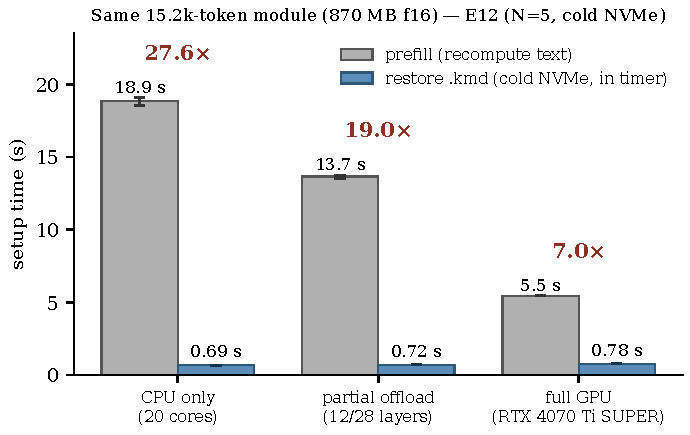
\includegraphics[width=0.62\linewidth]{fig-regimes.pdf}
  \caption{E12 compute-regime sweep ($N{=}5$ runs; bars are medians, whiskers min--max). The same 15.2k-token module on the same machine: prefill cost scales with available compute while restore cost is a flat, relocation-bound byte copy, so the precompilation advantage (7.0--27.6$\times$) peaks exactly where compute is scarce. Restore is read cold from NVMe (page cache evicted each run) with the \kmd{} read included in the timer; its ${<}2\,\%$ spread shows the cost is dominated by state relocation into device memory, not disk I/O.}
  \label{fig:regimes}
\end{figure}

Recall is 6/6 in every cell and every one of the five runs. Restore time is essentially flat across regimes (rising only slightly toward full GPU as more state is uploaded to the device) --- it is a relocation-bound byte copy, not a compute --- while prefill cost tracks available compute; the ratio therefore \emph{grows} exactly where compute is scarce. Nor does the flat restore depend on the module being cached in RAM: evicting the \kmd{} from the OS page cache before each timed restore (\code{posix\_fadvise(DONTNEED)}, eviction verified by the file read slowing to NVMe speed) adds only ${\sim}0.1$\,s --- \textbf{0.78\,s cold vs 0.65\,s warm at full GPU} (cold 0.69/0.72/0.78\,s across the three regimes, $N{=}5$, ${<}2\,\%$ spread) --- because the upload and scatter of state into device memory dominates the cost, not the disk read. On NVMe-class storage, modules can be served directly from cold disk with no warm-up; slower media (HDD, network) would reintroduce an I/O term. One honest caveat: a 20-core desktop CPU still prefills a 7B at ${\sim}800$\,t/s, so ``minutes vs milliseconds'' claims require weaker CPUs (machine A's laptop-class CPU prefills at an order of magnitude fewer t/s), larger models, or longer memories; the scaling direction, however, is unambiguous and multiplicative in all three factors. For the home-lab agent with a large persistent memory --- the setting that motivated this work --- precompilation is not an optimization but the difference between feasible and not.

\paragraph{The 51.8k-token point (E14).}
Scaling the E8 generator ${\sim}10\times$ (440 microservices across 11 regions plus 120 incidents, 51{,}790 tokens; seeded generator in \code{e14.py}) probes the length regime \S\ref{sec:limitations} previously listed as untested, on Qwen3-4B with the module read from disk inside the setup timer. Two dtype arms, each using the same cache type in \emph{every} condition: q8\_0 --- joint 31/60, linked \textbf{34/60}, no-memory 0/60, setup 2.62\,s vs 15.89\,s (\textbf{6.1$\times$}, up from 1.7$\times$ at 5.1k tokens on this GPU); f16 --- joint 29/60, linked \textbf{32/60}, setup 4.79\,s vs 13.85\,s (the larger 7.6\,GB module doubles link I/O relative to q8\_0's 4.1\,GB: at multi-GB module sizes the KV dtype directly buys link speed). Three observations. First, the linked module again never scores below joint prefill --- ${\sim}90\,\%$ of failures are shared between conditions, the E8 signature of a task-level (not insertion-level) limit. Second, the absolute drop (from 85\,\% at 5.1k to ${\sim}52$--$57\,\%$ here, failures concentrated on the most confusable attribute across 440 services) afflicts joint prefill equally: it is an interference/capacity property of the model at this scale, and the f16 arm matching q8\_0 rules out a quantized-cache cliff (extending \S\ref{sec:dtype}'s tolerance map for Qwen3-4B to 50k) --- an ablation that was mandatory before attributing the cause, since \S\ref{sec:dtype}'s cliffs produce exactly this plausible-but-wrong failure mode. The parity claim at 50k is therefore ``linking adds no cost'', not ``recall stays high'' --- though \S\ref{sec:cvm} shows the interference itself is removable: reading the same document page by page under a 4k budget recovers 49/60. Third, an ABI consequence: at this length the FA-off configuration used elsewhere in the paper stops being viable on a 16\,GB GPU --- without flash attention the materialized KQ scratch alone overflows VRAM (measured), and llama.cpp rejects quantized V caches without FA --- so long-memory modules will in practice use the FA-on ABI (\S\ref{sec:axes}).

\subsection{Multi-module workspace at 33k tokens and lazy loading at scale (E11)}
\label{sec:workspace}

The composition recipe of \S\ref{sec:compose} (first module linked whole; each subsequent module spliced with $k = 33\,\%$ recomputed) applied to all three E10 memories at once, on Qwen3-4B (q4 cache, 40k context): a \textbf{33.4k-token workspace assembled from three precompiled modules} versus joint prefill of the same tokens. All 120 questions:

\begin{table}[h]
  \centering\small
  \caption{E11: three-module workspace vs.\ joint prefill.}
  \begin{tabular}{lcc}
    \toprule
    Condition & Recall & Setup \\
    \midrule
    joint (33.4k prefill) & 105/120 & 9.25\,s \\
    workspace (1 link + 2 splice-$k$) & \textbf{106/120} & 8.18\,s (1.13$\times$) \\
    \bottomrule
  \end{tabular}
\end{table}

Composition at 20$\times$ the scale of \S\ref{sec:compose} is statistically indistinguishable from joint prefill (McNemar exact $p=1.0$, 95\,\% CI on the joint$-$workspace difference $[-7.9, +6.2]$\,pp over 120 paired questions) --- the powered counterpart to the underpowered \S\ref{sec:compose} micro-benchmark. The setup advantage nearly vanishes on this GPU --- splice-$k$ recomputes ${\sim}6.1$k tokens and the linker reads 1.39\,GB from disk --- so at datacenter-class compute the workspace pays in \emph{quality-preserving modularity}, not setup time; on consumer hardware the \S\ref{sec:regimes} regime arithmetic applies.

\paragraph{Lazy loading at scale.}
With only the 15.2k-token memory linked, six questions about the 10.2k-token memory score 0/6 (confirming inter-module isolation --- no leakage); linking that module mid-session (splice-$k$, 424\,MB from disk) takes \textbf{1.13\,s}, after which the same six questions score \textbf{6/6}. The \S\ref{sec:lazy} classloader pattern survives a 35$\times$ increase in loaded-module size with sub-second-scale latency.

\subsection{Speculative decoding over restored state: the MTP draft head (E13)}
\label{sec:mtp}

Current model families increasingly ship a \textbf{multi-token-prediction (MTP) draft head} --- an extra transformer block used for self-speculative decoding (DeepSeek-V3-style). This creates a compatibility question this section answers: does restoring precompiled KV state silently \emph{break} speculation on such models?

\paragraph{The gap.}
In llama.cpp, the MTP draft context shares KV cells with the target context (the upstream \code{[TAG\_KV\_CACHE\_SHARE\_CELLS]} mechanism), and for such shared-cell caches every state function is an unconditional no-op --- saving a draft context produces an empty blob and restoring reports success while writing nothing. The consequence is invisible by design: after a restore, the target model answers correctly (it verifies every speculated token), but the draft head attends over uninitialized KV for all restored positions, so acceptance drops and generation slows. We close the gap with a \textbf{${\sim}120$-line patch to the runtime library} (\code{llama-kv-cache.\{h,cpp\}}, included in the repository under \code{patches/}): serialize only the layers the draft cache \emph{owns}, and on restore --- target first, draft second --- locate the shared cells by position instead of allocating. Non-shared caches are byte-identical to the original code path.

\paragraph{E13.}
Qwopus3.5-4B-Coder-MTP Q6\_K (a GDN hybrid, 32 blocks + 1 MTP block --- one model exercising both \S\ref{sec:hybrid} and this section), 1{,}284-token memory, 43-token question, 120 greedy tokens, draft depth 2, each phase on a cold server process (machine B, CUDA):

\begin{table}[h]
  \centering\small
  \caption{E13: MTP speculative decoding over restored state.}
  \begin{tabular}{lccc}
    \toprule
    Condition & Prompt tokens processed & Draft acceptance & Gen.\ speed \\
    \midrule
    Full prefill (baseline) & 1{,}327 & 0.690 (69/100) & 203.7\,t/s \\
    Restore target + draft (patched) & \textbf{43} & \textbf{0.722 (70/97)} & 207.2\,t/s \\
    Restore, draft blob ablated (control) & 43 & 0.587 (64/109) & 185.2\,t/s \\
    \bottomrule
  \end{tabular}
\end{table}

Acceptance over restored state matches the full-prefill baseline; ablating \emph{only} the draft-head blob (5.0\,MB, vs.\ 90.4\,MB of target state) degrades acceptance and costs 9\,\% generation throughput while answers remain correct in all conditions --- a causal demonstration that the serialized draft state is what preserves speculation. Two full reruns reproduce every acceptance ratio and token count exactly (greedy decoding); wall-clock throughput varies within ${\sim}1\,\%$ run-to-run (e.g.\ 207.1 vs.\ 207.2\,t/s restored), so the t/s figures above are from one run. The draft blob is thus a \textbf{correctness-neutral optional payload}: a runtime that cannot ingest it loses only speed, never answers --- the right degradation semantics for a portable module section.

\paragraph{Two methodological traps worth reporting.}
Both initially masked the result behind a silent full re-prefill of the restored state. First, saving state one generated token past the memory boundary makes the follow-up request need a one-token rollback --- impossible for the hybrid's recurrent state, so the server silently reprocesses everything. Second, BPE merging across the memory/question boundary breaks the token-prefix match even when the \emph{text} is a prefix; the fix is cutting prompts at the exact common token prefix (token-array requests). With both fixed, the server extends restored hybrid state without re-prefill (43 tokens processed instead of 1{,}327) --- which also corrects a belief we held mid-investigation: hybrid slot restore is not broken, merely \emph{fragile}, failing silently on any boundary mismatch.

\subsection{Sliding-window attention: the linker inherits the model's visibility (E20)}
\label{sec:swa}

The last untested attention family within reach was interleaved sliding-window attention (SWA). On Gemma 3 4B (34 layers, 5 local : 1 global, window 1024 tokens), the full pipeline --- compile, serialize, restore, non-prefix link behind the adversarial ${\sim}1$k prefix, RoPE rebase --- runs \textbf{unmodified} on llama.cpp's iSWA cache. Recall parity with joint prefill is exact when the module is commensurate with the window ($16/20 = 16/20$ short-prefix; $15/25 = 15/25$ under the adversarial prefix; no-memory floors 0/20 and 5/25). With the 4.6k-token E8 memory --- 4.5$\times$ the window --- recall collapses \emph{symmetrically} (joint 16/60, linked 14/60, no-memory 0/60): only the global layers see the whole memory, and attribute binding across 40 services fails under prefill and linking alike. The linked module therefore inherits the model's own visibility semantics --- whatever the window would not have seen under joint prefill is equally unseen when linked --- so the operative rule for a memory manager is simple: modules at or below the SWA window come for free; larger ones return what the model itself returns at that distance. Two-module composition shows the familiar \S\ref{sec:compose} attribution deficit (18 vs 14 of 20; the splice-$k$ repair is untested here). Storage economics improve: SWA layers serialize only their window, so the module costs 47\,KB/token versus ${\sim}136$ for an equally-sized full-attention module of this class (215.8\,MB for 4{,}593 tokens) --- sublinear in document length for the local layers.

\section{Module ABI and a runtime-agnostic format}
\label{sec:abi}

\subsection{Compatibility axes}
\label{sec:axes}

Measured or derived from code, a module is compatible with a linking context only along five axes:

\begin{enumerate}
  \item \textbf{Exact model weights} --- the module is a function of them; any weight update invalidates it.
  \item \textbf{Tokenizer} --- the stored token ids must re-tokenize identically.
  \item \textbf{KV-cache dtype} --- the serialized tensor bytes must match the context's cache type (\S\ref{sec:dtype}).
  \item \textbf{V layout}: \code{v\_trans = !flash\_attn} --- the same command line can yield incompatible layouts on different GPUs under \code{-fa auto}, so FA must be pinned and recorded. Length forces the choice: at ${\sim}50$k tokens FA-off is not viable on a 16\,GB GPU (\S\ref{sec:regimes}, E14), so long-memory modules will in practice standardize on the FA-on layout (the \code{convert} operation of \S\ref{sec:kmd} bridges the two).
  \item \textbf{Backend is \emph{not} an axis} --- proven empirically (\S\ref{sec:phasea}, \S\ref{sec:regimes}): the same blob restores across Vulkan/CUDA/CPU.
\end{enumerate}

llama.cpp validates only architecture name and per-layer shapes; nothing binds a module to its source text or exact weights --- a stale module loads \emph{silently}. A production format must therefore carry \code{\{hash(weights), hash(tokenizer), hash(source MD), n\_tokens, tokens[], kv\_dtype, layout flags, format version\}}, making module identity content-addressed and staleness detectable --- the moral equivalent of solving Java's classpath hell up front.

\subsection{KV dtype: free compression until a silent cliff (E6)}
\label{sec:dtype}

\mdc{} supports all nine llama.cpp cache types; module sizes scale as predicted (f16 $\to$ q8\_0 0.53$\times$; q4\_0/iq4\_nl 0.28$\times$) and position rebasing over \emph{quantized} K (dequant $\to$ Hadamard $\to$ RoPE $\to$ requant) works end-to-end. A full E1-style battery per dtype on Qwen3-4B (E6: joint/linked at f16, f16+FA, q8\_0, q5\_1, q4\_0, iq4\_nl) shows every cell in the 17--18/20 noise band: at this scale, KV quantization down to 4-bit costs nothing measurable, the linked module never scores below joint prefill at any dtype, and FA on/off has no quality effect --- modules get 3.6$\times$ smaller for free.

This does \textbf{not} generalize unconditionally: the tolerance is model- and scale-dependent. Qwen3-4B holds q4\_0 KV up to 15k tokens (E10), but Qwen2.5-Coder-7B degenerates completely with a q4\_0 cache at ${\sim}9$k tokens (0/8 recall, repetitive output) while f16 is unaffected (7/8) --- and the failure applies to \emph{any} q4 cache, joint prefill included, so it is a property of the model$\times$dtype$\times$length combination, not of linking. A dtype sweep on the same bench places the cliff precisely: q8\_0 matches f16 (7/8 both), while q5\_1 already fails (0/8) --- and fails \emph{silently}, producing plausible but wrong numbers rather than degenerate text.

\textbf{Resulting production policy: q8\_0 as the default module dtype} (half of f16 for free), with sub-q8 dtypes admitted only after per-model, per-target-length validation. A production \mdc{} should automate that validation before compiling module stores.

\subsection{The \kmd{} container and the \mdc{} CLI}
\label{sec:kmd}

{\sloppy
We implement the content-addressed format as the \kmd{} v0 container and the \mdc{} CLI (\path{src/kmd/mdc.py}, installable via \code{pip install .}): \code{compile} with make-style staleness semantics; \code{index} (compiles a memory index plus all its \code{[[linked]]} MDs, warning on broken references); \code{verify} (detects stale source and wrong model without loading weights); \code{link} (the \S\ref{sec:compose} splice-$k$ production recipe built in); and \code{convert} (the FA$\leftrightarrow$non-FA layout transposition of \S\ref{sec:background}, byte-identical on round-trip).\par}

Hybrid models are first-class: \code{compile} detects the architecture from GGUF metadata, runs the per-layer probes, and attaches the $T_M$ matrices plus RoPE parameters (needed because e.g.\ Qwen3.5-2B rotates only 64 of its 256 head dimensions) under a \code{hybrid} header; \code{link --recr naive|affine} applies the software rebase and the chosen state policy.

Module size is \emph{not} stable across models: bytes/token = layers $\times$ GQA-KV width $\times$ dtype size, and token count varies by tokenizer --- measured 147.5\,KB/token (Qwen3-4B), ${\sim}109$ (Llama-3.2-3B), ${\sim}57$ (Qwen2.5-Coder-7B, whose 4-head GQA makes its modules 2.6$\times$ smaller than the 4B's). Weight quantization does not affect module size at all; only the KV dtype does.

\subsection{Toward a runtime-agnostic interchange format (E9)}
\label{sec:interchange}

Because the mathematical content (per-layer, per-token K/V plus positions) depends only on (model, tokenizer, text, RoPE policy) and not on the serving engine, a canonical layout-neutral interchange format with per-runtime loaders (scatter into llama.cpp cell rows or vLLM 16-token paged blocks) is feasible --- ELF/ONNX-style. vLLM integration additionally requires extending the scheduler-connector contract, which is prefix-shaped today --- in fact narrower: the stock disk connector (E9) keys storage by a hash of the \emph{entire prompt}, so KV is not reused even across different questions over the same memory. E9 nevertheless replicates the Phase-A result (\S\ref{sec:phasea}) inside vLLM v1 with it: restored-KV answers are token-identical to full prefill (5/5 recall both) at 2.4$\times$ TTFT on an RTX 4070 Ti SUPER --- the precompile/restore contract holds in a second, architecturally unrelated runtime. The required engine surface is small: MiniPIC \citep{ordonez2026} demonstrates PIC primitives in a vLLM fork with under 100 lines of core-engine changes, which strengthens the case that the missing piece is a contract, not a rewrite. The MTP result of \S\ref{sec:mtp} sharpens the contrast between engine designs: vLLM registers MTP/EAGLE draft layers as first-class groups in its unified KV-cache manager, addressable by layer name through the same connector interface --- so the draft section of a module needs \emph{no} engine change there (the draft KV's one-position offset, which vLLM handles via its ``last-block drop'' rule, is a convention the interchange format must record), whereas llama.cpp's shared-cell design required the \S\ref{sec:mtp} serialization fix. The thickness of a per-runtime loader is a property of the engine's API surface, not of the format.

\subsection{Beyond memories: skills, plans, and tool catalogs}
\label{sec:skills}

The module abstraction is not specific to memories. Most of what surrounds an agent's context window is static, versioned text that is re-prefilled ritually on every session: skill definitions (SKILL.md), project conventions (AGENTS.md), standing plans (PLAN.md), and --- the heaviest in practice --- \emph{tool catalogs}. Tools are declared as JSON Schemas but reach the model as ordinary tokens in the system prompt; an MCP-connected session routinely carries tens of thousands of tokens of schema text before the first user word (we observed ${\sim}23$k tokens of active tool schemas, plus ${>}100$k deferred, in a production coding-agent session).

These artifacts are \emph{better} compilation candidates than memories along every axis of \S\ref{sec:axes}: they are identical across users and sessions (compile once, amortize arbitrarily widely), centrally versioned (content-addressed identity is the natural fit), and increasingly loaded \emph{on demand} --- a skill invoked mid-conversation, a deferred tool schema fetched when first needed. On-demand loading is precisely non-prefix insertion: the artifact arrives after an unpredictable conversation prefix, exactly the case prefix caching cannot serve (\S\ref{sec:phasea}) and the linker exists for (\S\ref{sec:compose}--\S\ref{sec:lazy}). The lazy-loading protocol of \S\ref{sec:lazy}/\S\ref{sec:workspace} maps one-to-one onto skill and tool loading, with one simplification available for free in an agentic loop: because new tokens attend causally to everything before them, a model that defers its answer until after the tool result --- the standard tool-use pattern --- needs no re-question step at all: link the module when the tool returns, then generate.

\subsection{Persistence by reference}
\label{sec:byref}

Linked modules break an implicit invariant of today's LLM applications: that the conversation transcript is self-contained --- that replaying its text reconstructs the state. A module contributes KV state but no transcript text, so a session that linked one can only be faithfully resumed by a runtime able to re-link it: serialized conversations must store \emph{references} --- \code{\{module\_id, position\}} pairs --- rather than content, and the content-addressed identity of \S\ref{sec:axes} is exactly what such a reference needs (staleness and wrong-model detection included).

Two further system consequences follow. Context accounting must charge modules against the window even though they never appear as text --- a 500-word chat may hold a 33k-token workspace (\S\ref{sec:workspace}). And unloading is not symmetric with loading: evicting a module from the middle of a sequence requires rebasing everything after it, so eviction belongs between turns, under a manager with pinning (see the memory-manager design note in the repository, \code{docs/ARCHITECTURE.md}).

Both eviction paths are validated on live conversations (\code{e15.py}/\code{e15b.py}, findings H34 in the lab notebook). For full-attention models, in-place eviction plus compaction (\code{seq\_rm} of the module's cells, negative \code{seq\_add} over the tail) costs \textbf{0.5--1\,ms} --- the lazy K-shift lands on the next decode --- and is behaviorally neutral: over seven turns with six module switches, isolated-battery recall is identical with paging (22/42) and with everything resident (21/42), while the bounded working set halves peak cell usage (16k vs 34k). For GDN hybrids the recurrent accumulator cannot be truncated per-token (its ``eviction'' is undefined: the module's contribution cannot be factored out of the fold), so the manager uses \textbf{checkpoint-and-replay} --- a sequence-level snapshot before each link; on eviction, restore and re-decode only the post-module turns --- evicting in ${\sim}5$\,ms at $O(\text{tail})$, never $O(\text{module})$, cost (41/42 vs the no-eviction control's 39/42 on Qwen3.5-4B). In both cases the conversation \emph{keeps what was said}: answer tokens generated while a module was resident retain its content in their own KV rows (the model still quotes its first exchange verbatim after six compactions), so eviction loses only what was never asked. Finally, provenance: the model now ``knows'' content whose text never crossed the conversation, so the tool stub that links a module should declare the module's identity, keeping that knowledge auditable at the UI level.

\subsection{Context virtual memory}
\label{sec:cvm}

The eviction of \S\ref{sec:byref} plus one further primitive --- \textbf{sealing a range of the live conversation as an anonymous module} (\code{seq\_cp} of the range to a scratch sequence, serialize, evict and compact) --- completes the middle layer that \S\ref{sec:related} identified as vacant between MemGPT's text-level paging and PagedAttention's physical block paging: a virtual-memory hierarchy for the context itself, where page-out preserves exact state and page-in is the linker.

\paragraph{A conversation larger than the window (E16).}
With \code{n\_ctx} deliberately set to 4{,}096 and a watermark at 3{,}000 cells, a scripted 14-report conversation totalling \textbf{5{,}528 tokens} --- which would abort on context overflow without sealing --- ran to completion with 7 segments sealed to host RAM (244\,ms each, dominated by serializing 58\,MB). Isolation is exact: questions about sealed segments score 0/21 without page-in. Paging the sealed segment back (142\,ms) recovers \textbf{15/21 --- equal to or better than the 14/21 of segments that never left}. What bounds the conversation is no longer the window but storage; the resident working set is bounded by the watermark.

\paragraph{Paged reading of a 51.8k-token document under a 4k budget (E18).}
The E14 memory (identical generator, seed, and 60-question sample) was split at semantic boundaries into 28 chunks of ${\sim}2$k tokens and \textbf{compiled page by page: 51{,}790 tokens in 8.8\,s with \code{n\_ctx} never exceeding 4{,}096} --- the VRAM wall that \S\ref{sec:regimes}'s full-context run had to engineer around cannot occur by construction, and compilation is embarrassingly parallel. Reading uses a deterministic page table (the chunk containing the service or incident named by the question; selection and paging are thus measured separately --- a production selector adds its own error term) with a 109\,ms mean page-in:

\begin{table}[h]
  \centering\small
  \caption{E18: paged reading vs.\ the full-context reference (same memory, seed, and questions as E14).}
  \label{tab:paged}
  \begin{tabular}{lcc}
    \toprule
    Condition & Recall & n\_ctx \\
    \midrule
    Full-context prefill (E14 joint) & 31/60 & 57{,}344 \\
    Full-context link (E14 naive) & 34/60 & 57{,}344 \\
    \textbf{Paged, one chunk per question (E18)} & \textbf{49/60} & \textbf{4{,}096} \\
    \bottomrule
  \end{tabular}
\end{table}

Paging at this scale is not an accuracy trade-off \emph{once the correct page is selected}: it \emph{outscores} the full context by 15 points while using a 14$\times$ smaller window, because the model reads a 2k-token page containing the relevant facts instead of attending across 440 interfering entries (the capacity limit diagnosed in \S\ref{sec:regimes}). The residual failures are all one question template answered in the wrong format --- none are page misses. Two honest qualifiers: E18's page table is a deterministic \emph{oracle} that already knows which chunk holds each answer, so 49/60 is the ceiling a real selector (\S\ref{sec:cvm}) works toward, not the end-to-end number it would achieve; and this experiment prices only the page-in, not the full economics (per-chunk compilation, multi-GB module storage, and the break-even against selective \emph{text} retrieval), which we leave as future work. The result replicates across models: under the same 4k budget, Qwen2.5-Coder-7B scores 46/60 (44\,ms page-ins --- its 4-head GQA makes pages 2.6$\times$ lighter) and Qwen3-14B a \textbf{perfect 60/60} (full-context references at 51.8k exist only for the 4B; for the 14B, whose single-hop score at 5.1k was 57/60, paged reading of a 10$\times$ larger document is at ceiling).

\paragraph{Residency is not addressability.}
Across seven independent measurements in this paper --- E10 (twice), E14 (both dtype arms), E15b, E16, and E18 --- a freshly linked module in a small context never scored below, and usually scored above, the same content resident in a large one. We read this as: a large context window acts as an \emph{addressing} mechanism, not an attention guarantee --- recall degrades with resident interference even under joint prefill, and paging exact state into a small working set restores it. The honest boundaries: selection must be solved (E18's page table was deterministic), and tasks requiring cross-page synthesis --- multi-hop across chunks, whole-document summarization --- cannot be served from a single page and remain the adverse case for paging designs (within one module, two-hop questions cost joint prefill and linked modules equally: aggregate 73 vs 74 of 120 across three models, E17).

\section{Limitations}
\label{sec:limitations}

Small cells ($N{=}10$--$25$ per condition; $N{=}60$ in E8/E14, $N{=}120$ in E10/E11), nine small-to-mid instruction-tuned models (2B--14B), two GPUs plus a CPU point, synthetic Spanish-language memories, greedy decoding, substring-based scoring, and paired significance testing (McNemar exact, with Newcombe 95\,\% CIs) reported only on \emph{pooled} cells --- per-cell $N$s (10--60) are individually underpowered, so no single cell is significant in either direction, and the 10\,pp non-inferiority margin of \S\ref{sec:single} was fixed post hoc rather than pre-registered. A single synthetic factual-recall battery underlies the recall claims; more corpora, task types (instruction-following, reasoning, cross-span attribution), and module orderings/positions remain untested. The E2/E8 ``no deficit'' result is an absence of evidence at ${\sim}1$k-token prefixes and up-to-51.8k-token modules, not a proof; at 51.8k absolute recall drops for joint prefill and linked modules alike (\S\ref{sec:regimes}), so parity there means ``no added cost'', not ``high recall''. Two-hop questions within one module cost both conditions equally (aggregate 73 joint vs 74 linked of 120 across three models, E17), but with per-model variance in both directions (Coder-7B $-5$, Qwen3-14B $+6$ for the linked module; $N{=}40$ per cell) and multi-hop \emph{across} pages under the \S\ref{sec:cvm} paging regime remains untested. The \S\ref{sec:cvm} sealing result (E16) uses one model; the paged-reading result (E18) replicates on three (49, 46, and 60 of 60), but its page selector is deterministic --- a production selector adds its own error term. Module storage is heavy (f16 $\approx 147$\,KB/token for a 4B GQA model; ${\sim}36{,}000\times$ the source text) though cold storage is cheap and the q8\_0 default halves it --- and hybrid recurrent layers invert this economics (constant size per module). E7's naive/affine parity means the affine machinery, while numerically validated, has not yet been shown \emph{behaviorally} necessary (one hybrid family at three sizes, $\leq 1.3$k-token memories). M-RoPE and GDN hybrids joined the compatible set in \S\ref{sec:hybrid}, MTP draft heads in \S\ref{sec:mtp} (one model, one quantization, and --- unlike every other result --- requiring our library patch until it lands upstream), and interleaved SWA in \S\ref{sec:swa} (one model; beyond-window memories degrade equally under joint prefill and linking, and the splice-$k$ repair is untested there); MLA (DeepSeek-family latent attention) and multimodal caches remain outside it. Backend coverage is likewise two runtimes --- llama.cpp, whose downstream wrappers (Ollama, LM Studio, llamafile) inherit the mechanism unchanged, and vLLM, where our result is a prefix-restore feasibility check (E9, \S\ref{sec:interchange}) rather than a working non-prefix linker: importing a \code{.kmd}, non-prefix insertion, and running the linker inside vLLM all remain future work. Other major serving stacks also cache KV hierarchically (SGLang's HiCache \citep{zheng2024}, TensorRT-LLM's cache reuse) but, like vLLM's native connector, remain prefix-bound --- they reuse state produced by the engine's own execution rather than accepting relocatable external modules --- so extending the linker to them is future work, not an expected incompatibility.

\section{Future work}
\label{sec:future}

Smarter boundary recomputation (token selection by KV deviation à la CacheBlend, or by importance propagation à la KEEP, instead of a fixed prefix-$k$); extending the affine linker of \S\ref{sec:hybrid} to \emph{purely recurrent} models (Mamba/RWKV), where no attention layers exist to compensate and the affine policy is the only prefix-preserving mechanism --- the natural testbed its validated machinery still lacks; extending \mdc{}/\kmd{} v0 (implemented, \S\ref{sec:kmd}) with a layout-neutral cross-runtime profile and principled compression --- generic lossless compression is \emph{not} it: measured on real modules, zlib recovers only 7--13\,\% on f16 blobs (quantized ones are less compressible still) while capping restore at ${\sim}300$\,MB/s, far below NVMe; the productive levers are the KV dtype (q8\_0 halves size behaviorally free, \S\ref{sec:dtype}) and CacheGen-style lossy delta encoding; extending the \code{mtp} section of \kmd{} (implemented as format v1 --- modules package the patched server's target and draft state files with content-addressed identity, validated by byte-identical round-trip against the \S\ref{sec:mtp} artifacts) with draft-KV relocation and an in-process compile path, and upstreaming the serialization fix; a vLLM connector plus scheduler-contract extension (\S\ref{sec:interchange}); scaling studies beyond the 51.8k-token and 14B points measured in \S\ref{sec:single}/\S\ref{sec:regimes}, toward the regime where per-question recall itself becomes the bottleneck and paging designs apply; multi-hop question workloads; and multi-module workspaces with dozens of lazily-loaded memories beyond the three of \S\ref{sec:workspace}.

\section{Conclusion}
\label{sec:conclusion}

Treating agent memories as precompiled, relocatable, composable KV modules is not a speculative architecture: on stock llama.cpp binaries, single-module insertion at arbitrary positions shows no statistically detectable recall difference from joint prefill at every scale we tested (1.4k--15.2k tokens; pooled McNemar $p=0.69$, 95\,\% CI on the deficit within $\pm3$\,pp), a three-module 33k-token workspace matches joint prefill ($p=1.0$), lazy mid-session loading works at a 1\,s cost, and the one quality gap found --- multi-module attribution --- is reduced by recomputing a third of the inserted module at negligible cost, closing to joint-prefill parity at workspace scale. The setup advantage ranges from 7.0$\times$ on a discrete GPU to 27.6$\times$ on CPU for the same 15k-token memory, growing exactly where compute is scarce --- consumer and edge hardware. The approach is not even confined to pure-attention transformers: the same linker extends to linear-attention hybrids, where a memory module becomes a constant-size affine operator on the recurrent state --- arguably a more natural ``compiled memory'' than per-token KV, and a capability no serving-side caching system currently offers. What distinguishes this work from the concurrent PIC line is not the relocation trick but the \emph{object model}: KV state promoted from cache entry to artifact --- persistent, portable across machines and backends, content-addressed, staleness-checked --- compiled where compute is cheap and linked where it is scarce. The missing system component in today's runtimes is the linker, and this work shows it can be built from primitives they already ship.

\section*{Acknowledgments}

The implementation, experiment execution, and drafting of this paper were carried out with substantial assistance from Claude (Anthropic), used as a research and engineering tool under the author's direction. All experimental claims are backed by the raw outputs versioned in the accompanying repository and are independently reproducible with the scripts provided.

\begin{thebibliography}{99}\small

\bibitem[Gim et al.(2024)]{gim2024}
Gim, I., Chen, G., Lee, S.-s., Sarda, N., Khandelwal, A., and Zhong, L. (2024).
\emph{Prompt Cache: Modular Attention Reuse for Low-Latency Inference.}
Proceedings of MLSys 2024. arXiv:2311.04934.

\bibitem[Hu et al.(2025)]{hu2025}
Hu, J., Huang, W., Wang, W., Wang, H., Hu, T., Zhang, Q., Feng, H., Chen, X., Shan, Y., and Xie, T. (2025).
\emph{EPIC: Efficient Position-Independent Caching for Serving Large Language Models.}
Proceedings of ICML 2025. arXiv:2410.15332.

\bibitem[Kwon et al.(2023)]{kwon2023}
Kwon, W., Li, Z., Zhuang, S., Sheng, Y., Zheng, L., Yu, C. H., Gonzalez, J. E., Zhang, H., and Stoica, I. (2023).
\emph{Efficient Memory Management for Large Language Model Serving with PagedAttention.}
Proceedings of SOSP 2023. arXiv:2309.06180.

\bibitem[Liu et al.(2024)]{liu2024}
Liu, Y., Li, H., Cheng, Y., Ray, S., Huang, Y., Zhang, Q., Du, K., Yao, J., Lu, S., Ananthanarayanan, G., Maire, M., Hoffmann, H., Holtzman, A., and Jiang, J. (2024).
\emph{CacheGen: KV Cache Compression and Streaming for Fast Large Language Model Serving.}
Proceedings of ACM SIGCOMM 2024. arXiv:2310.07240.

\bibitem[LMCache Team(2024)]{lmcache2024}
LMCache Team (2024).
\emph{LMCache: An Efficient KV Cache Layer for Enterprise-Scale LLM Inference.}
Software, \url{https://github.com/LMCache/LMCache}.

\bibitem[Ordonez and Parnell(2026)]{ordonez2026}
Ordonez, N., and Parnell, T. (2026).
\emph{MiniPIC: Flexible Position-Independent Caching in {\textless}100 LOC.}
arXiv:2606.13126.

\bibitem[Packer et al.(2023)]{packer2023}
Packer, C., Wooders, S., Lin, K., Fang, V., Patil, S. G., Stoica, I., and Gonzalez, J. E. (2023).
\emph{MemGPT: Towards LLMs as Operating Systems.}
arXiv:2310.08560.

\bibitem[Qin et al.(2025)]{qin2025}
Qin, R., Li, Z., He, W., Zhang, M., Wu, Y., Zheng, W., and Xu, X. (2025).
\emph{Mooncake: A KVCache-centric Disaggregated Architecture for LLM Serving.}
Proceedings of USENIX FAST 2025. arXiv:2407.00079.

\bibitem[Xiao et al.(2024)]{xiao2024}
Xiao, G., Tian, Y., Chen, B., Han, S., and Lewis, M. (2024).
\emph{Efficient Streaming Language Models with Attention Sinks.}
Proceedings of ICLR 2024. arXiv:2309.17453.

\bibitem[Yang et al.(2025a)]{yangj2025}
Yang, J., Hou, B., Wei, W., Bao, Y., and Chang, S. (2025).
\emph{KVLink: Accelerating Large Language Models via Efficient KV Cache Reuse.}
NeurIPS 2025. arXiv:2502.16002.

\bibitem[Yang et al.(2025b)]{yangs2025}
Yang, S., Kautz, J., and Hatamizadeh, A. (2025).
\emph{Gated Delta Networks: Improving Mamba2 with Delta Rule.}
Proceedings of ICLR 2025. arXiv:2412.06464.

\bibitem[Yang et al.(2026)]{yangz2026}
Yang, Z., Xie, T., Lu, B., Liu, S., Yu, B., and Li, M. (2026).
\emph{KEEP: A KV-Cache-Centric Memory Management System for Efficient Embodied Planning.}
Proceedings of DAC 2026. arXiv:2602.23592.

\bibitem[Yao et al.(2025)]{yao2025}
Yao, J., Li, H., Liu, Y., Ray, S., Cheng, Y., Zhang, Q., Du, K., Lu, S., and Jiang, J. (2025).
\emph{CacheBlend: Fast Large Language Model Serving for RAG with Cached Knowledge Fusion.}
Proceedings of EuroSys 2025. arXiv:2405.16444.

\bibitem[Ye et al.(2025)]{ye2025}
Ye, H., Gao, Z., Ma, M., Wang, Q., Fu, Y., Chung, M.-Y., Lin, Y., Liu, Z., Zhang, J., Zhuo, D., and Chen, Y. (2025).
\emph{KVCOMM: Online Cross-context KV-cache Communication for Efficient LLM-based Multi-agent Systems.}
Proceedings of NeurIPS 2025. arXiv:2510.12872.

\bibitem[Zheng et al.(2024)]{zheng2024}
Zheng, L., Yin, L., Xie, Z., Sun, C. L., Huang, J., Yu, C. H., Cao, S., Kozyrakis, C., Stoica, I., Gonzalez, J. E., Barrett, C., and Sheng, Y. (2024).
\emph{SGLang: Efficient Execution of Structured Language Model Programs.}
Proceedings of NeurIPS 2024. arXiv:2312.07104.

\end{thebibliography}

\section*{Reproducibility}

All scripts and raw results live in the accompanying public repository, \url{https://github.com/k0n1m4k1/kv-memory-modules}:

\begin{itemize}\sloppy
  \item \textbf{Investigation notebook}: \code{docs/NOTEBOOK.md} (H1--H42), the lab record behind every claim (Spanish original in \code{docs/NOTEBOOK.es.md}).
  \item \textbf{Core tooling} (\code{src/kmd/}, installable via \code{pip install .}): \code{llamalib.py} (ctypes bindings), \code{mdc.py} (\kmd{} v0 compiler/linker CLI, including \code{convert} and hybrid modules), \code{hyblib.py} (hybrid/GDN support), \code{linker.py} (original Phase-B harness).
  \item \textbf{Experiment batteries} (\code{experiments/}): \code{bateria.py}--\code{bateria6.py} (E1--E6, E8), \code{bateria7.py}/\code{bateria8.py}/\code{e12.py} (E10--E12 including the cold-NVMe arm, shared helpers in \code{common.py}), \code{hibrido0.py}--\code{hibrido4.py} (E7 and follow-ups), \code{fase3\_vllm.py} (E9), \code{e13v2.py} (E13, run against the patched build), \code{e14.py} (E14, seeded 51.8k-token generator), \code{e15.py}/\code{e15b.py} (live eviction/compaction on conversations, \S\ref{sec:byref}), \code{e16.py}/\code{e18.py} (context virtual memory: sealing and paged reading, \S\ref{sec:cvm}), \code{e17.py} (two-hop battery), \code{gen\_corpus.py} (seeded E10 corpus generator, seed 20260719), plus the Phase-A server scripts \code{scripts/run-poc*.ps1}. E20 (SWA, \S\ref{sec:swa}) is \code{bateria2.py} and \code{bateria6.py} re-run unmodified on Gemma-3-4B-it; E19 (vLLM MTP) is \code{e19.py}. Paired significance analysis (McNemar exact + Newcombe 95\,\% CIs, \S\ref{sec:single}/\S\ref{sec:compose}/\S\ref{sec:workspace}) is \code{stats\_recall.py}, run offline over the versioned \code{results/} JSON --- no model or GPU required.
  \item \textbf{Runtime patches} (\code{patches/}, E13 only): \path{llama.cpp-b10068-mtp-kv-state-shared-cells.patch} (library fix, upstream candidate) and \path{llama.cpp-b10068-server-slots-draft-state.patch} (experimental server companion); apply instructions in \code{patches/README.md}. Every other experiment uses unmodified b10068 binaries.
  \item \textbf{Raw outputs}: \code{results/resultados-*.json} (one JSON per battery run, versioned).
  \item \textbf{Test corpora} (\code{data/}): \code{memoria-agente.md}, \code{memoria-general.md}, \code{memoria-ancla.md}, \code{system-agente.md}, \code{prefijo-largo.md}, and the generated \code{memoria-hist/tec/ops.md} with \code{preguntas-e10.json}.
  \item \textbf{Environment}: bootstrap via \code{scripts/setup-linux.sh} / \code{scripts/setup-windows.ps1}; full suite via \code{scripts/run-suite.sh}; summary viewer \code{scripts/show-results.py}. llama.cpp release b10068 (machine A: official win-vulkan-x64 binaries; machine B: built from source with CUDA); vLLM 0.22.1 for E9.
  \item \textbf{Machines}: A = Windows 11, Intel Arc 140V 16\,GB (Vulkan); B = Ubuntu 24.04, RTX 4070 Ti SUPER 16\,GB, 20-core CPU (CUDA).
  \item \textbf{Models}: see Appendix~\ref{app:models} and \code{scripts/models.txt}.
\end{itemize}

\appendix

\section{Models}
\label{app:models}

All experiments use GGUF builds served by llama.cpp b10068 (E9 uses the safetensors release under vLLM). Module compatibility is bound to the \emph{exact} GGUF file (weights hash, \S\ref{sec:axes}), so the table records the specific quantized build used. ``KV dtypes used'' lists the cache/module dtypes each model was measured with.

\begin{landscape}
\begin{table}[p]
  \centering\footnotesize
  \setlength{\tabcolsep}{5pt}
  \caption{Models used in the evaluation. GGUF sources are Hugging Face repositories.}
  \label{tab:models}
  \begin{tabular}{p{3.4cm}p{6.2cm}cp{1.5cm}p{4.4cm}>{\raggedright\arraybackslash}p{4.6cm}}
    \toprule
    Model & Architecture & Layers & Weights (GGUF) & KV dtypes used & GGUF source \\
    \midrule
    Qwen3-4B-Instruct-2507 & Dense, full attention, GQA (8 KV heads), 262k ctx & 36 & Q4\_K\_M & f16, q8\_0, q5\_1, q4\_0, iq4\_nl (E6); q4\_0 at 15k (E10); f16/q8\_0 with FA at 51.8k (E14) & \path{unsloth/Qwen3-4B-Instruct-2507-GGUF} \\
    Llama-3.2-3B-Instruct & Dense, full attention, GQA & 28 & Q4\_K\_M & f16 & \path{unsloth/Llama-3.2-3B-Instruct-GGUF} \\
    Qwen2.5-Coder-7B-Instruct & Dense, full attention, GQA (4 KV heads), code-specialized & 28 & Q4\_K\_M & f16, q8\_0 (q5\_1/q4\_0 collapse at ${\sim}9$k, \S\ref{sec:dtype}) & \path{Qwen/Qwen2.5-Coder-7B-Instruct-GGUF} \\
    Qwen3-14B & Dense, full attention, GQA (8 KV heads) & 40 & Q4\_K\_M & f16 & \path{unsloth/Qwen3-14B-GGUF} \\
    Qwen3.5-2B & Hybrid: Gated DeltaNet 3:1 (18 GDN + 6 gated-attention M-RoPE layers), 262k ctx & 24 & Q4\_K\_M & f16 attention + f32 recurrent state & \path{unsloth/Qwen3.5-2B-GGUF} \\
    Qwen3.5-4B & Hybrid: Gated DeltaNet 3:1 (24 GDN + 8 attention layers) & 32 & Q4\_K\_M & f16 + f32 recurrent & \path{unsloth/Qwen3.5-4B-GGUF} \\
    Qwen3.5-9B & Hybrid: Gated DeltaNet 3:1 (recurrent state 32 heads $\times$ $128 \times 128$ per layer) & 32 & Q8\_0 & f16 + f32 recurrent & \path{unsloth/Qwen3.5-9B-GGUF} \\
    Qwopus3.5-4B-Coder-MTP & Hybrid: Gated DeltaNet 3:1 + embedded MTP draft block (\code{qwen35} arch, 32+1 blocks); coding fine-tune of Qwen3.5-4B & 33 & Q6\_K & f16 (target + draft state blobs) & \path{Jackrong/Qwopus3.5-4B-Coder-MTP-GGUF} \\
    Gemma-3-4B-it & Dense, interleaved SWA 5 local : 1 global (window 1024, GQA 4 KV heads), 128k ctx & 34 & Q4\_K\_M & f16 (SWA layers serialize only their window: 47\,KB/token measured) & \path{ggml-org/gemma-3-4b-it-GGUF} \\
    \bottomrule
  \end{tabular}
\end{table}
\end{landscape}

{\sloppy
Model cards: each GGUF repository above links its base model card (\path{Qwen/Qwen3-4B-Instruct-2507}, \path{meta-llama/Llama-3.2-3B-Instruct}, \path{Qwen/Qwen2.5-Coder-7B-Instruct}, \path{Qwen/Qwen3-14B}, \path{Qwen/Qwen3.5-2B}, \path{Qwen/Qwen3.5-4B} --- also the base of the Qwopus coding fine-tune, Apache 2.0 --- \path{Qwen/Qwen3.5-9B}, and \path{google/gemma-3-4b-it}) at \path{https://huggingface.co/<repo>}. Exact file names and download commands: \code{scripts/models.txt} and \code{scripts/setup-linux.sh}.\par}

\end{document}
